\chapter{Materials and Methods}

This chapter details the materials and methods used for the development of this work. Initially, the materials employed are described, including specific equipment, light sources, calibration patterns, and software used for data acquisition, processing, and analysis.

Subsequently, the experimental methods are presented, organized according to the type of measurement performed: geometric and spectral measurements. For each method, the experimental procedure is clearly described, justifying the choice of technique and specifying the conditions under which the experiments were conducted, including details of instrument configuration and protocols followed.


% Finalmente, se incluye una breve descripción de los resultados esperados tras la ejecución de los métodos mencionados, acompañada del cronograma previsto para las actividades y el presupuesto estimado requerido para la implementación del estudio. Esta información busca proporcionar claridad y facilitar la replicabilidad del estudio, así como sustentar la factibilidad y pertinencia metodológica del proyecto.


% \section{Parámetros Espectrales para la Determinación de Índices de Vegetación}

% Para una caracterización efectiva y la calibración de cámaras multiespectrales destinadas a la medición de índices de vegetación, es crucial considerar los siguientes parámetros espectrales:

% \subsection{Sensibilidad Espectral del Sensor}
% \begin{itemize}
%     \item \textbf{Rango Espectral}: Define las longitudes de onda a las que el sensor es sensible. Para la mayoría de las aplicaciones en vegetación, es esencial cubrir desde el espectro visible (400-700 nm) hasta el infrarrojo cercano (700-1100 nm). Esta sensibilidad permite la detección precisa de la reflectancia de la vegetación, lo cual es crítico para índices como el NDVI \cite{Huang2021ASensing}.
%     \item \textbf{Sensibilidad Relativa}: Mide la respuesta del sensor a diferentes longitudes de onda dentro del rango espectral. La sensibilidad relativa determina qué tan bien el sensor puede diferenciar entre diversas características de la vegetación basándose en sus firmas espectrales \cite{Dale2013HyperspectralReview, Klein2011MethodsCameras}.
% \end{itemize}

% \subsection{Transmisión Espectral del Objetivo (Lente)}
% \begin{itemize}
%     \item \textbf{Coeficiente de Transmisión Espectral}: Este parámetro describe la proporción de luz transmitida a través del objetivo en función de la longitud de onda. Es fundamental evaluar cómo los objetivos afectan la intensidad y calidad de la luz que llega al sensor para evitar distorsiones espectrales que puedan afectar la precisión de los índices de vegetación \cite{Xue2017SignificantApplications}.
%     \item \textbf{Rango de Transmisión Espectral}: El objetivo debe permitir la transmisión efectiva de las longitudes de onda relevantes (por ejemplo, bandas roja e infrarroja cercana) utilizadas para el cálculo de índices de vegetación. El rango de transmisión afecta directamente la calidad de la señal recibida por el sensor \cite{Dale2013HyperspectralReview}.
% \end{itemize}

% \subsection{Características Espectrales del Filtro}
% \begin{itemize}
%     \item \textbf{Curva de Transmitancia Espectral}: Define cómo el filtro permite o bloquea diferentes longitudes de onda. Es esencial para asegurar que sólo las longitudes de onda deseadas alcancen el sensor, eliminando posibles interferencias de otras bandas espectrales \cite{Huang2021ASensing}.
%     \item \textbf{Longitud de Onda de Corte y Ancho de Banda de Transmisión}: La longitud de onda de corte indica el punto donde el filtro comienza a bloquear la luz, mientras que el ancho de banda de transmisión especifica el rango de longitudes de onda que el filtro permite pasar. Estos parámetros son clave para seleccionar y diferenciar bandas espectrales específicas necesarias para índices de vegetación \cite{Dale2013HyperspectralReview}.
% \end{itemize}

% \subsection{Respuesta Espectral Combinada del Sistema}
% \begin{itemize}
%     \item \textbf{Eficiencia Espectral Total}: Considera la eficiencia combinada de sensor, objetivo y filtro para captar la luz en las longitudes de onda relevantes. Esto incluye la integración de todas las respuestas espectrales de los componentes individuales para determinar la capacidad del sistema completo en la detección y medición de índices de vegetación \cite{Xue2017SignificantApplications}.
%     \item \textbf{Linealidad y Estabilidad Espectral}: Evalúa cómo se mantiene la respuesta espectral del sistema bajo diferentes condiciones de iluminación y ambientales. La estabilidad espectral es crítica para aplicaciones en campo donde las condiciones pueden variar significativamente \cite{Dale2013HyperspectralReview}.
% \end{itemize}

% Estos parámetros deben ser cuidadosamente caracterizados y calibrados para asegurar que la cámara multiespectral proporcione datos precisos y fiables para la medición de índices de vegetación, facilitando así aplicaciones como el monitoreo de la salud de los cultivos, la evaluación del estrés vegetal y el análisis de cambios en la cobertura vegetal.


\section{Geometric Characterization}

\subsubsection{Determination of Field of View (FOV) and Angular Field of View (AFOV)}
\label{sec:fov}

The Field of View (FOV) of the optical system is determined in order to assess the maximum angle of the scene that the camera can capture. First, a test film is placed on a stable base located on the optical bench, preferably using a clamp that allows proper orientation with respect to the optical axis of the system. It is essential that the film is properly positioned to minimize errors caused by tilts or misalignments.

Next, the optical system is positioned on its corresponding base on the optical bench, ensuring it is centered and properly aligned with the test film (see Figure~\ref{fig:MTF_FOV_montage}). Once the initial setup is established, images of the film are captured at different working distances. During image acquisition, an effort is made to precisely align the visible edges of the image with a known edge on the test film. Measurements are taken strictly in the vertical or horizontal direction, explicitly measuring the distance between objects located at opposite edges of the image. This procedure is carried out for both the horizontal and vertical FOV, as they may differ depending on the format of the optical sensor.

\begin{figure}[H]
        \centering
        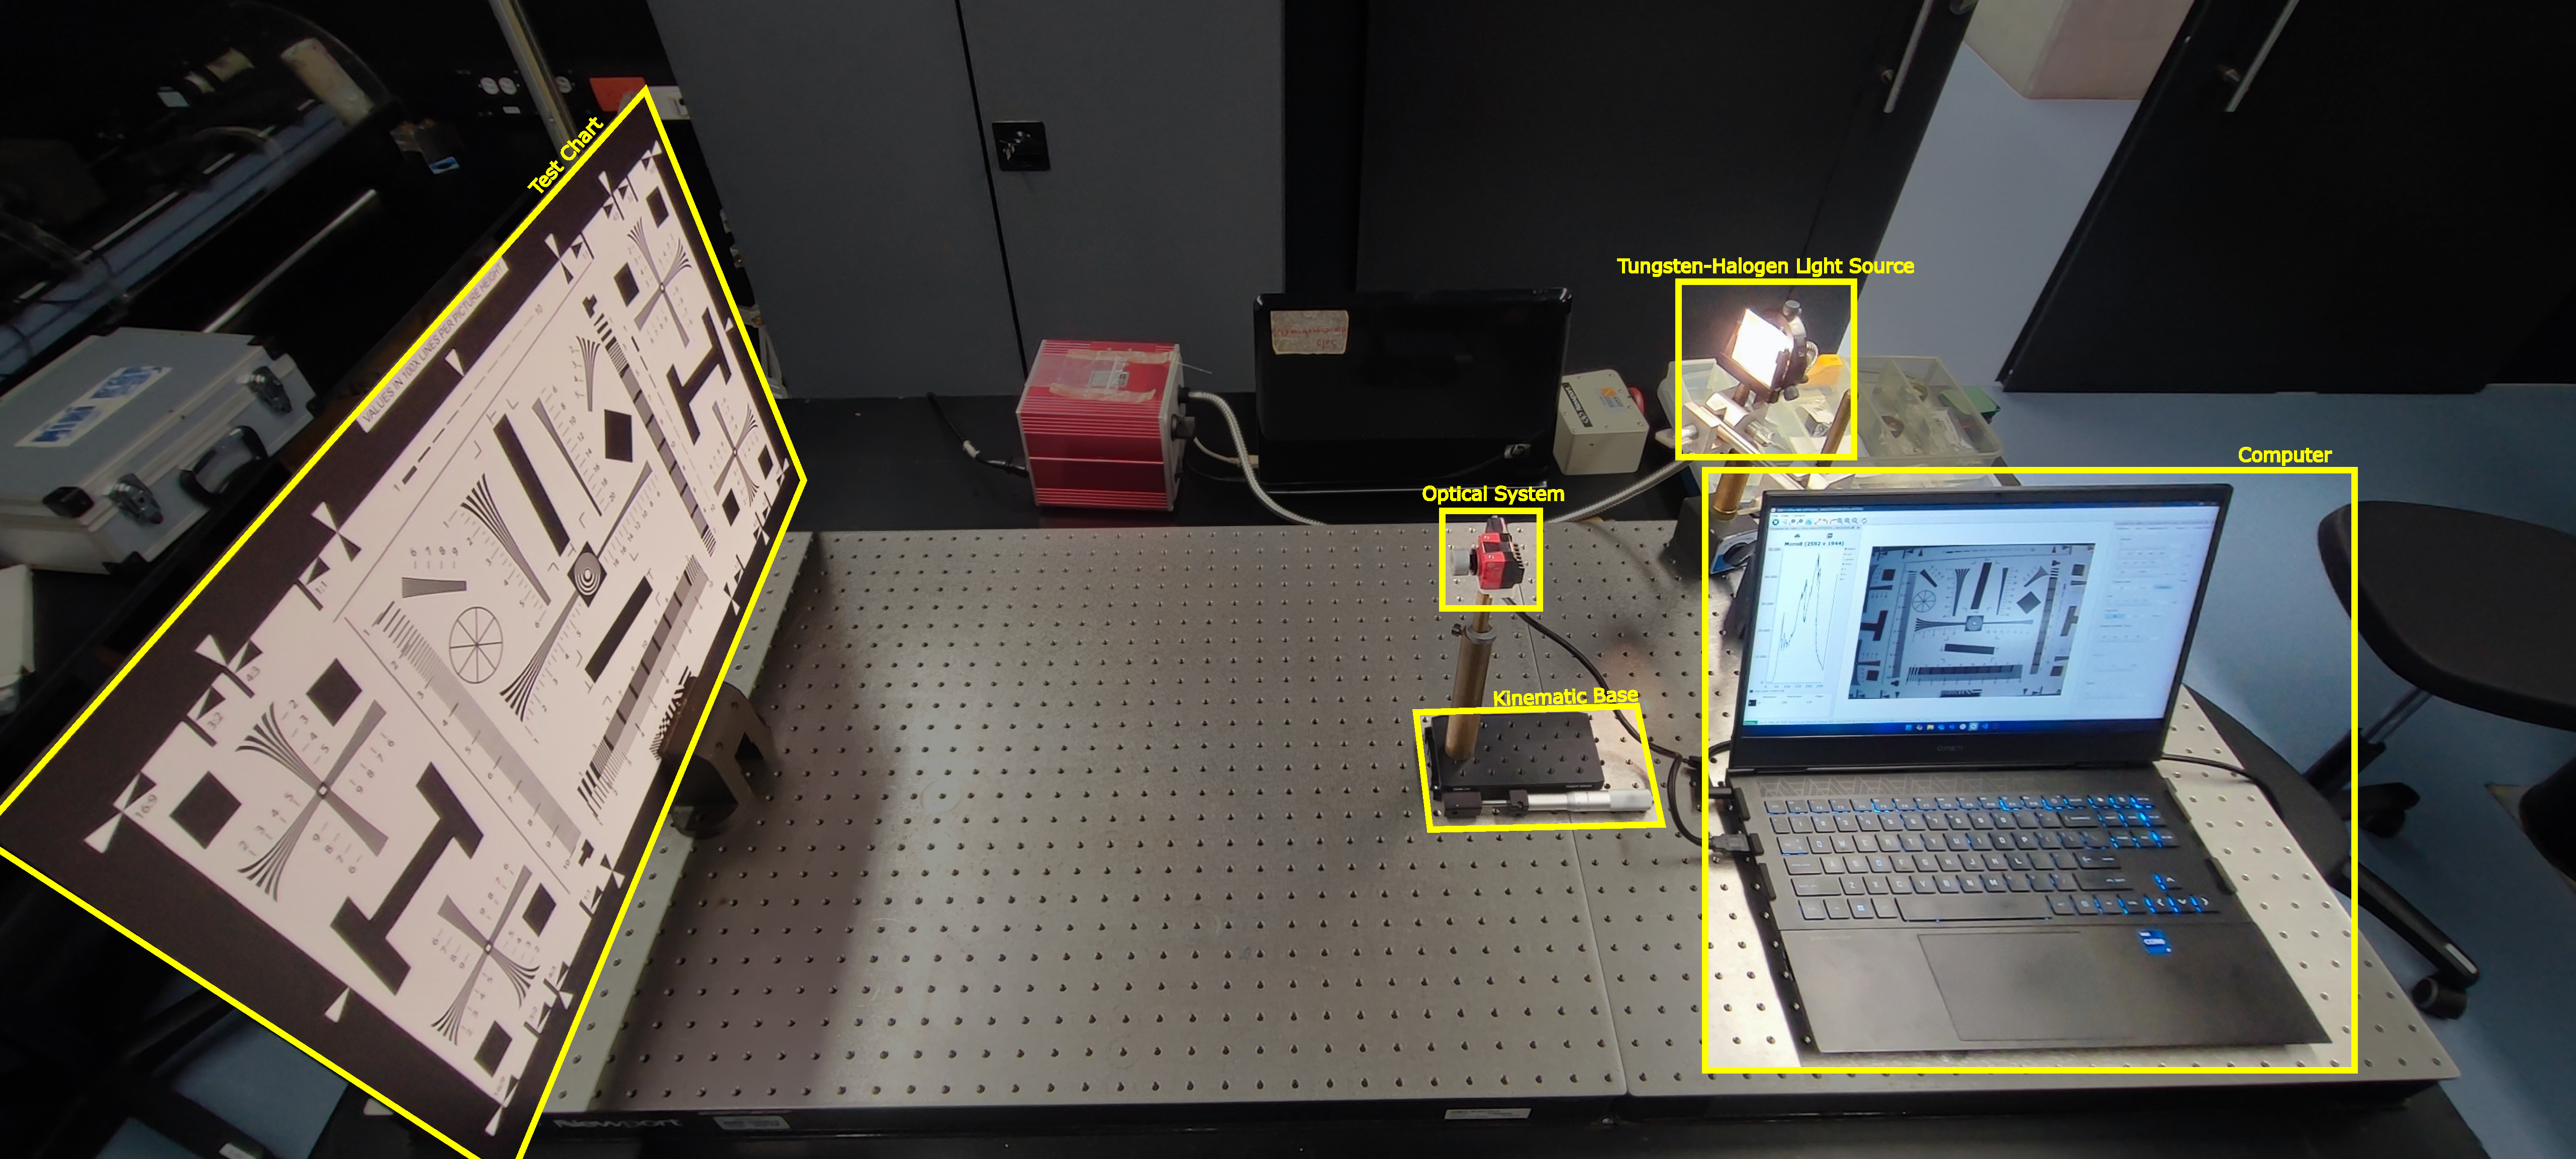
\includegraphics[width=0.8\linewidth]{Figures/C3/MTF_montaje.pdf}
        \caption{Optical setup developed. In this case, the use of barriers to prevent capture of unwanted light directly from the illumination source was not necessary, as the source is located behind the optical system under test. The illumination source is a tungsten halogen lamp coupled with a fiber optic cable and a diffuser.}
        \label{fig:MTF_FOV_montage}
\end{figure}

Since FOV measurements have inherent uncertainties due to the measuring instrument and other experimental sources, a statistical analysis using weighted linear regression is implemented to properly model the functional relationship between the measured FOV and the working distance. This method explicitly considers errors in both the dependent and independent variables, allowing for consistent and less biased estimates of the model parameters. The weighted linear regression is fitted using total least squares (Deming regression), which simultaneously minimizes deviations in both variables:

\begin{equation}
\text{FOV} = \beta_1 \cdot \text{Working distance} + \beta_0,
\label{eq:regresion_lineal}
\end{equation}

where \( \beta_1 \) is the slope and \( \beta_0 \) is the intercept, both calculated along with their associated uncertainties, thus ensuring a statistically reliable model to describe the behavior of the FOV as a function of working distance.

To minimize errors introduced by optical aberrations, such as spherical aberration, the measurements are preferably taken along the central vertical axis of the image. Specialized Python software is then used to analyze the images and calculate the angular FOV using the geometric relation:

\begin{equation}
\text{AFOV} = 2 \cdot \arctan\left(\frac{\text{FOV}}{2 \cdot d}\right),
\label{eq:fov_angular}
\end{equation}

where \( d \) is the working distance.\\

Regarding the system's focusing, it is recommended to use an autofocus mechanism for proper image acquisition of the test chart. Since the optical systems used in this study have a fixed focal length, the focus must be manually adjusted to obtain a high-quality image. To optimize this adjustment, a method is used based on capturing an image of a well-defined edge, from which the corresponding intensity profile is extracted and displayed in real-time, in this case along the central horizontal line. The derivative of this profile is then calculated and plotted to represent the intensity variation across the edge transition. Focus optimization is achieved by maximizing the prominence of the peak in the derivative, indicating a higher definition in the signal variation. This point of maximum variation is considered indicative of correct focus. Figure~\ref{fig:enfoque_conjunta} shows a representative example of optimal edge focusing.

\begin{figure}[H]
    \centering
    % First subfigure
    \begin{subfigure}[b]{0.7\linewidth}
        \centering
        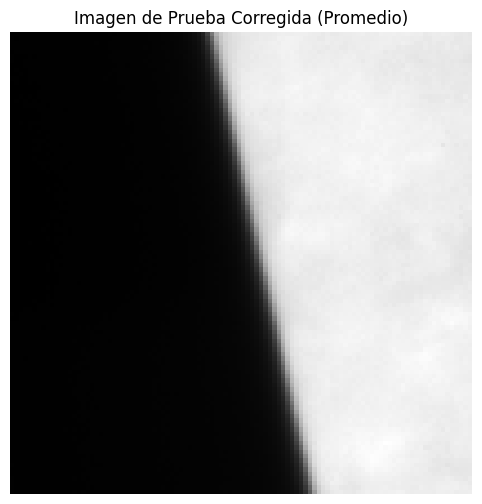
\includegraphics[trim=0mm 0mm 0mm 10mm, clip, width=\linewidth]{Figures/C3/SE_1.png}
        \caption{Image of an edge, used to properly adjust the optical system focus.}
        \label{fig:enfoque}
    \end{subfigure}
    
    \vspace{1em} % Vertical space between subfigures

    % Second subfigure
    \begin{subfigure}[b]{0.95\linewidth}
        \centering
        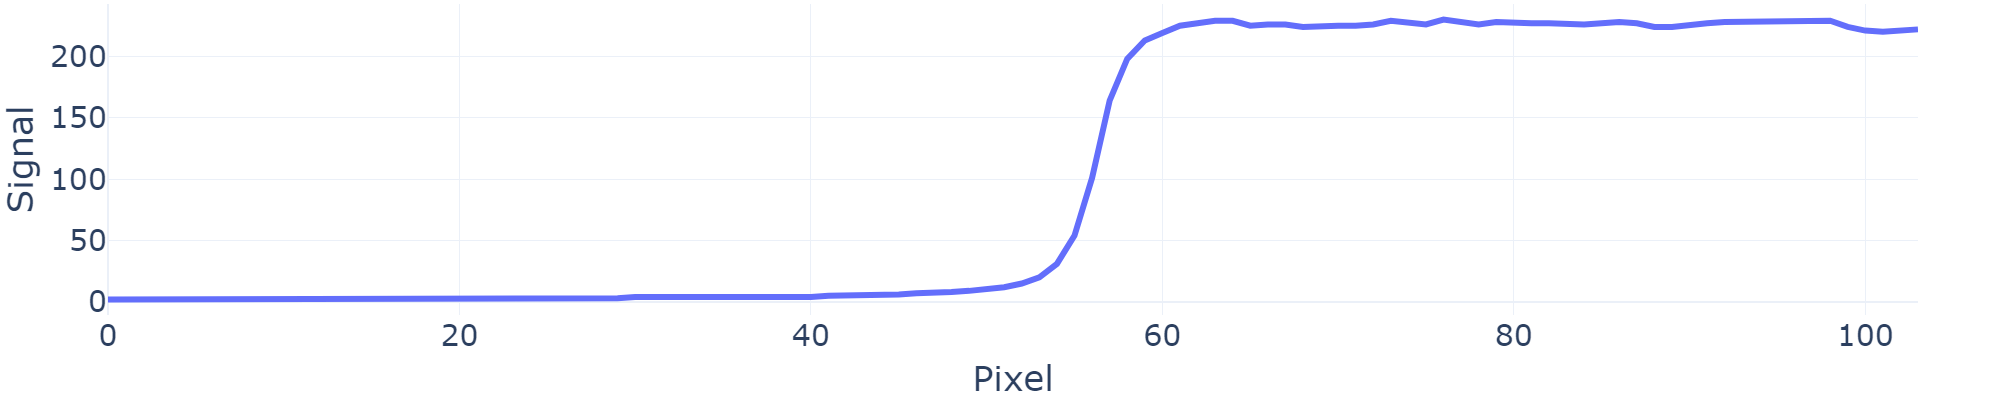
\includegraphics[width=\linewidth]{Figures/C3/SE_signal.png}
        \caption{Central profile of the edge image.}
        \label{fig:se_signal}
    \end{subfigure}
    
    \vspace{1em} % Vertical space between subfigures

    % Third subfigure
    \begin{subfigure}[b]{0.95\linewidth}
        \centering
        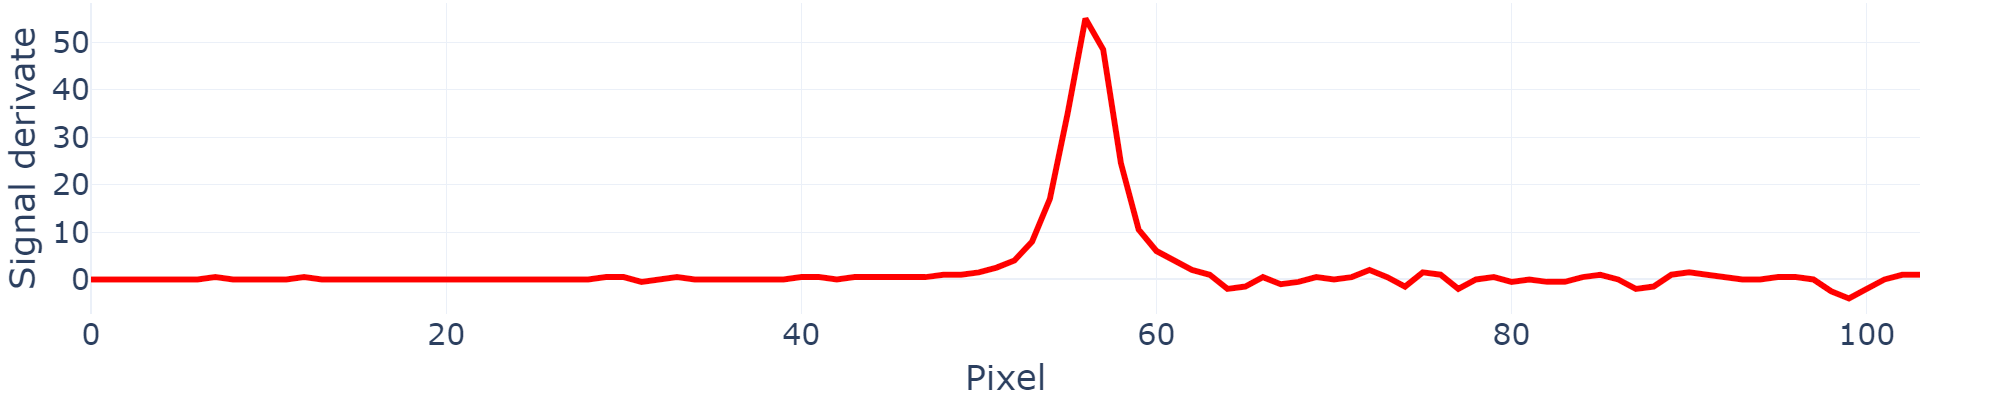
\includegraphics[width=\linewidth]{Figures/C3/SE_diff.png}
        \caption{Derivative of the central profile.}
        \label{fig:se_diff}
    \end{subfigure}
    
    \caption{Set of images with their corresponding profile and derivative.}
    \label{fig:enfoque_conjunta}
\end{figure}

\subsection{Modulation Transfer Function (MTF) Characterization}

The Modulation Transfer Function (MTF) enables an objective evaluation of the optical system’s ability to reproduce detail and contrast at different spatial frequencies. In this work, the slanted-edge method is used, as established by the international standard ISO 12233, which offers high precision, repeatability, and reliability.

The procedure begins by placing the ISO 12233 standard spatial resolution chart (see Figure~\ref{fig:iso12233_test_chart}) on a stable base. Uniform illumination over the chart’s surface is ensured, guaranteeing that the light intensity at any point does not vary more than $\pm 10\%$ from the center value. To prevent direct light from hitting the optical system, barriers are installed to block any undesired light.

\begin{figure}[H]
    \centering
    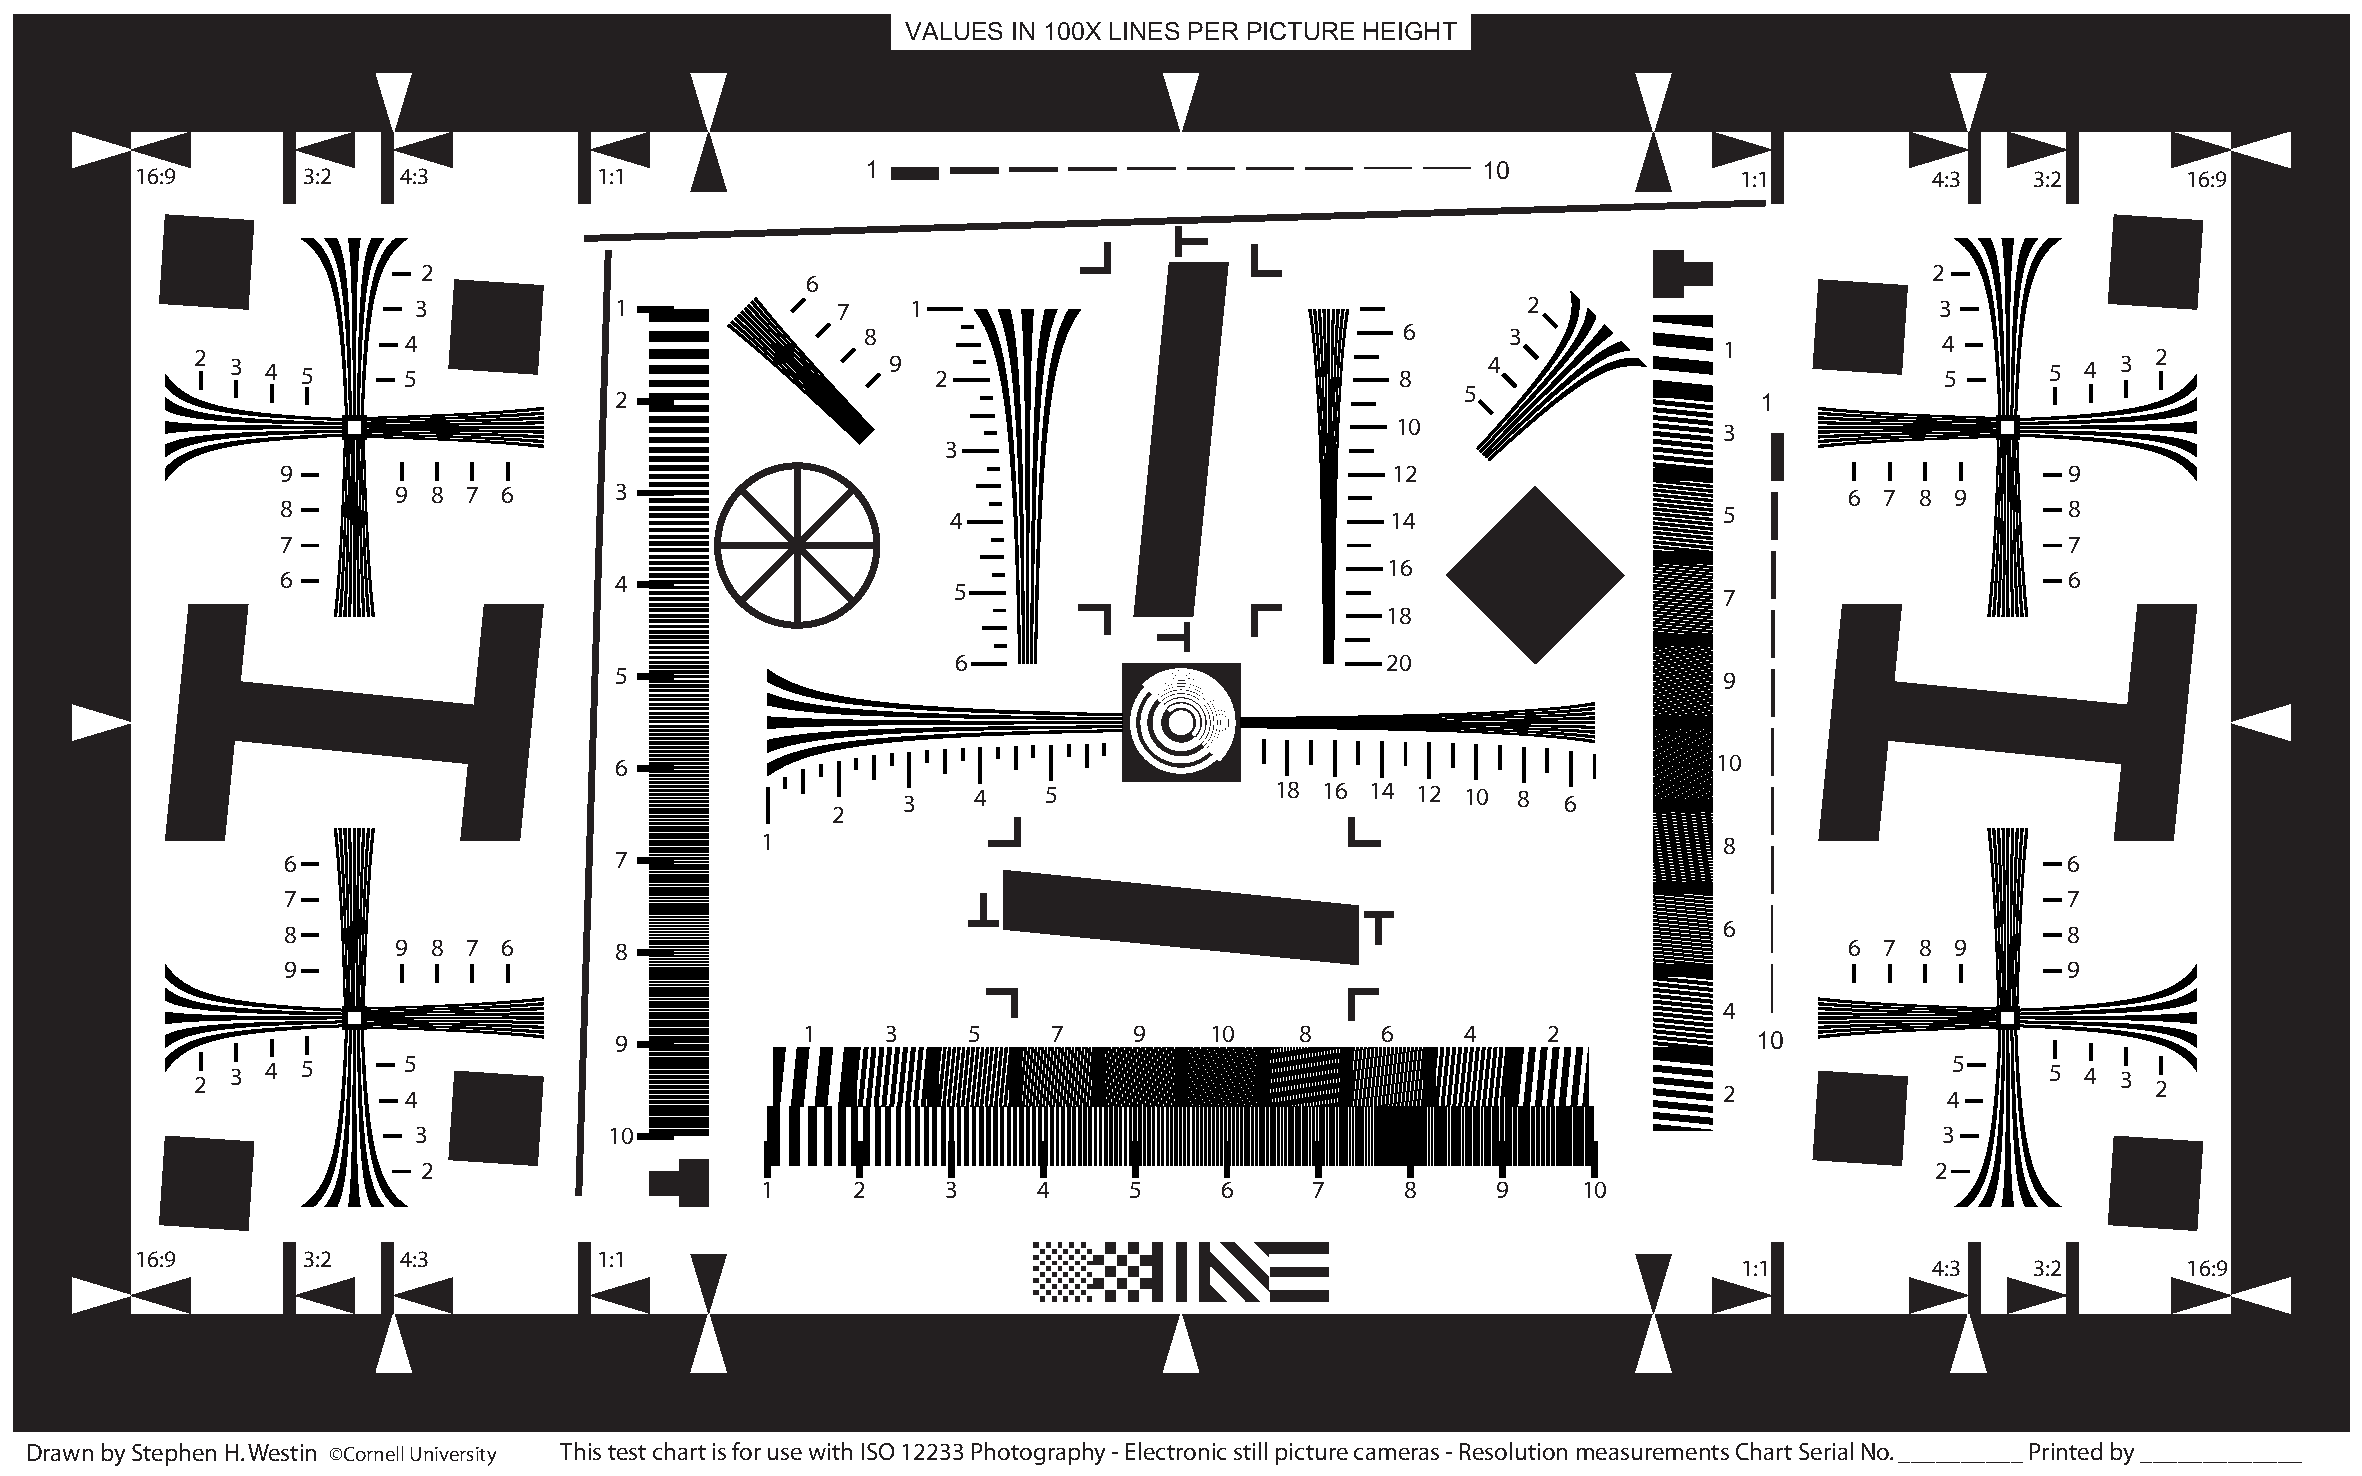
\includegraphics[width=0.95\linewidth]{Figures/C3/ISO_12233-reschart.pdf}
    \caption{Standard chart used to measure the spatial frequency response of the optical system, as established in the ISO 12233 standard.}
    \label{fig:iso12233_test_chart}
\end{figure}

Since the optical system under analysis does not have autofocus and instead requires manual adjustment, a Python script was implemented to display the camera or sensor image in real time, along with a window showing the central horizontal intensity profile and another window showing its derivative. To determine optimal focus, the method seeks to maximize the magnitude of the extreme values—peaks and valleys—of the derivative of the central profile, since a higher derivative corresponds to better edge resolution. This indicates that the focus point has been reached where high spatial frequency details are best reproduced. This method is the same as described in Section~\ref{sec:fov}.\\

The aperture and exposure time of the optical system are carefully adjusted to obtain a maximum signal without saturation in the bright areas of the target. Signal clipping must be avoided in both bright and dark regions, including the transition zones of the slanted edge. As image compression can significantly affect resolution measurements, all system settings must be recorded and reported, including focal length, aperture, sensor resolution, and compression modes used. When using color cameras, proper white balance must be applied according to the light source, as specified in ISO 14525. White balance may be performed automatically if the software and optical system support it, or manually using the RGB channel histogram. The goal is to overlap the histogram peaks of the three channels as much as possible. For this work, white balance was performed manually, ensuring that the peaks corresponding to the bright zone overlap across the three RGB channels. This signal distribution can be seen in Figure~\ref{fig:illumination_distribution}.\\

The MTF measurement is carried out following the steps outlined below:

\begin{enumerate}
    \item The illumination is configured as shown in Figure~\ref{fig:srf_motaje}. Ambient lighting must be reduced to a minimum. If necessary, a diffuser should be used to ensure the illumination is as homogeneous as possible and to avoid unwanted intensity patterns from the light source.
    
    \begin{figure}[H]
        \centering
        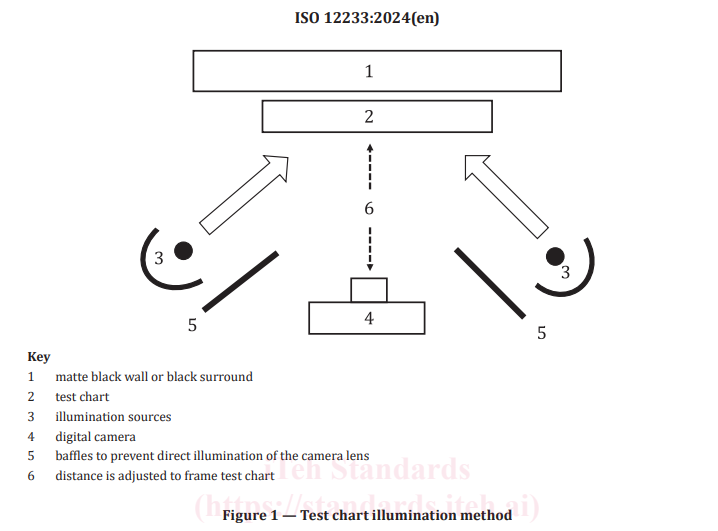
\includegraphics[trim=20mm 50mm 20mm 0mm, clip, width=0.7\linewidth]{Figures/C3/iso 12233 montaje.png}
        \caption{Optical setup recommended by ISO 12233:2024 for accurate MTF measurement. (1) matte black background, (2) test chart, (3) white illumination, (4) optical system under test, (5) barriers to prevent direct illumination of the optical system, (6) adjustable working distance.}
        \label{fig:srf_motaje}
    \end{figure}

    \item The illumination is arranged such that the signal distribution delivered by the optical system is as homogeneous as possible. This implies that the captured image should show two well-defined peaks: one for the dark areas and another for the bright areas of the test pattern. Ideally, these peaks would be delta functions, indicating sharp transitions between intensity regions. In practice, secondary peaks should be minimized and the main peaks should be as narrow as possible. A homogeneous distribution ensures the optical system’s response is measured under controlled conditions and the MTF analysis is not affected by unwanted illumination variations. Figure~\ref{fig:illumination_distribution} shows the distribution achieved for the region of interest shown in Figure~\ref{fig:enfoque}. Additionally, this distribution confirms that signal saturation is minimal in the region of interest.

    \begin{figure}[H]
        \centering
        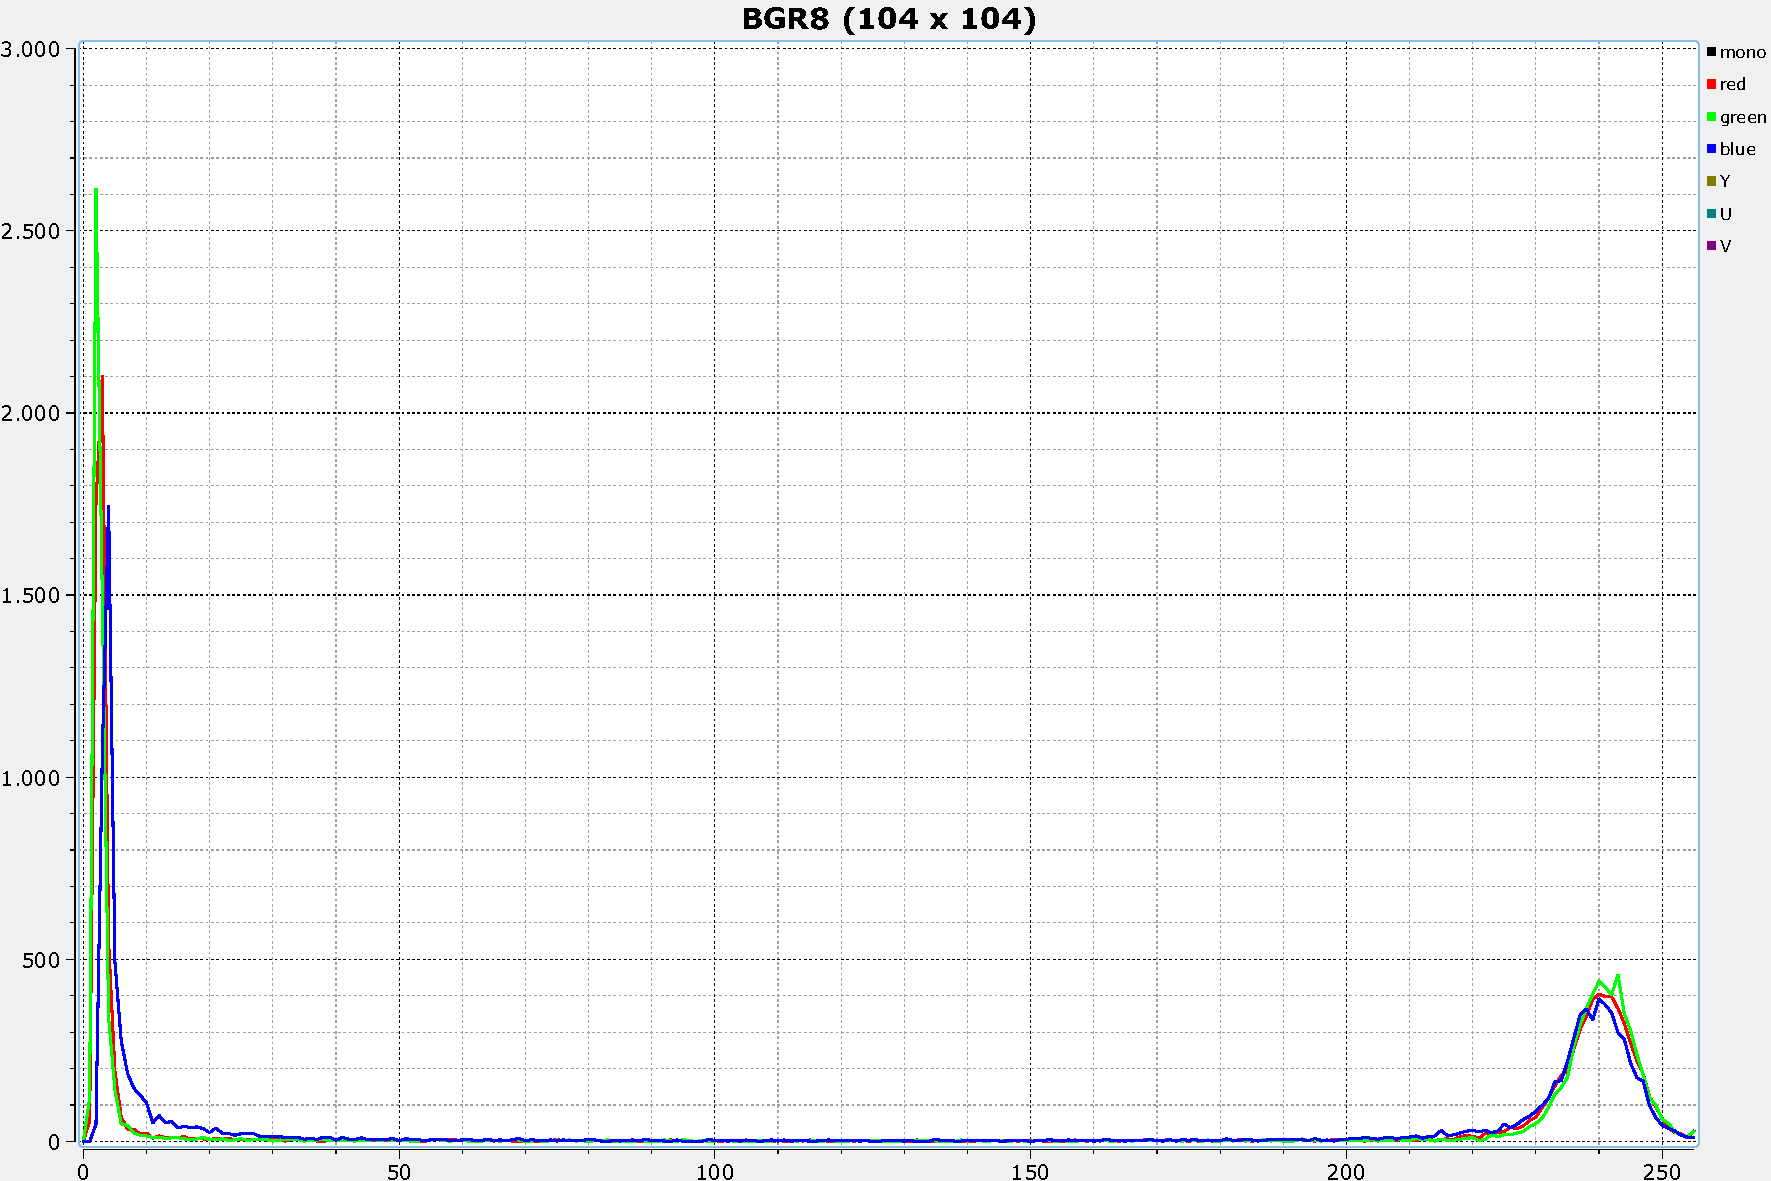
\includegraphics[width=1\linewidth]{Figures/C3/Histogram_MTF.pdf}
        \caption{Signal distribution delivered by the optical system under the configured experimental illumination. Two main peaks are observed: one in the dark zone and another in the bright zone, with attenuated secondary peaks.}
        \label{fig:illumination_distribution}
    \end{figure}

    \item The optical system is positioned to properly frame the test chart. Vertical arrows help adjust magnification, while horizontal arrows assist in centering the image. The tips of the central black arrows should be fully visible, while the white arrows should be completely hidden. The horizontal edge of the chart should be aligned approximately parallel to the sensor’s horizontal lines. The approximate distance between the camera and the test chart is recorded for later analysis. Figure~\ref{fig:iso12233_test_chart_encuadre} shows the arrows used for alignment.

    \begin{figure}[H]
        \centering
        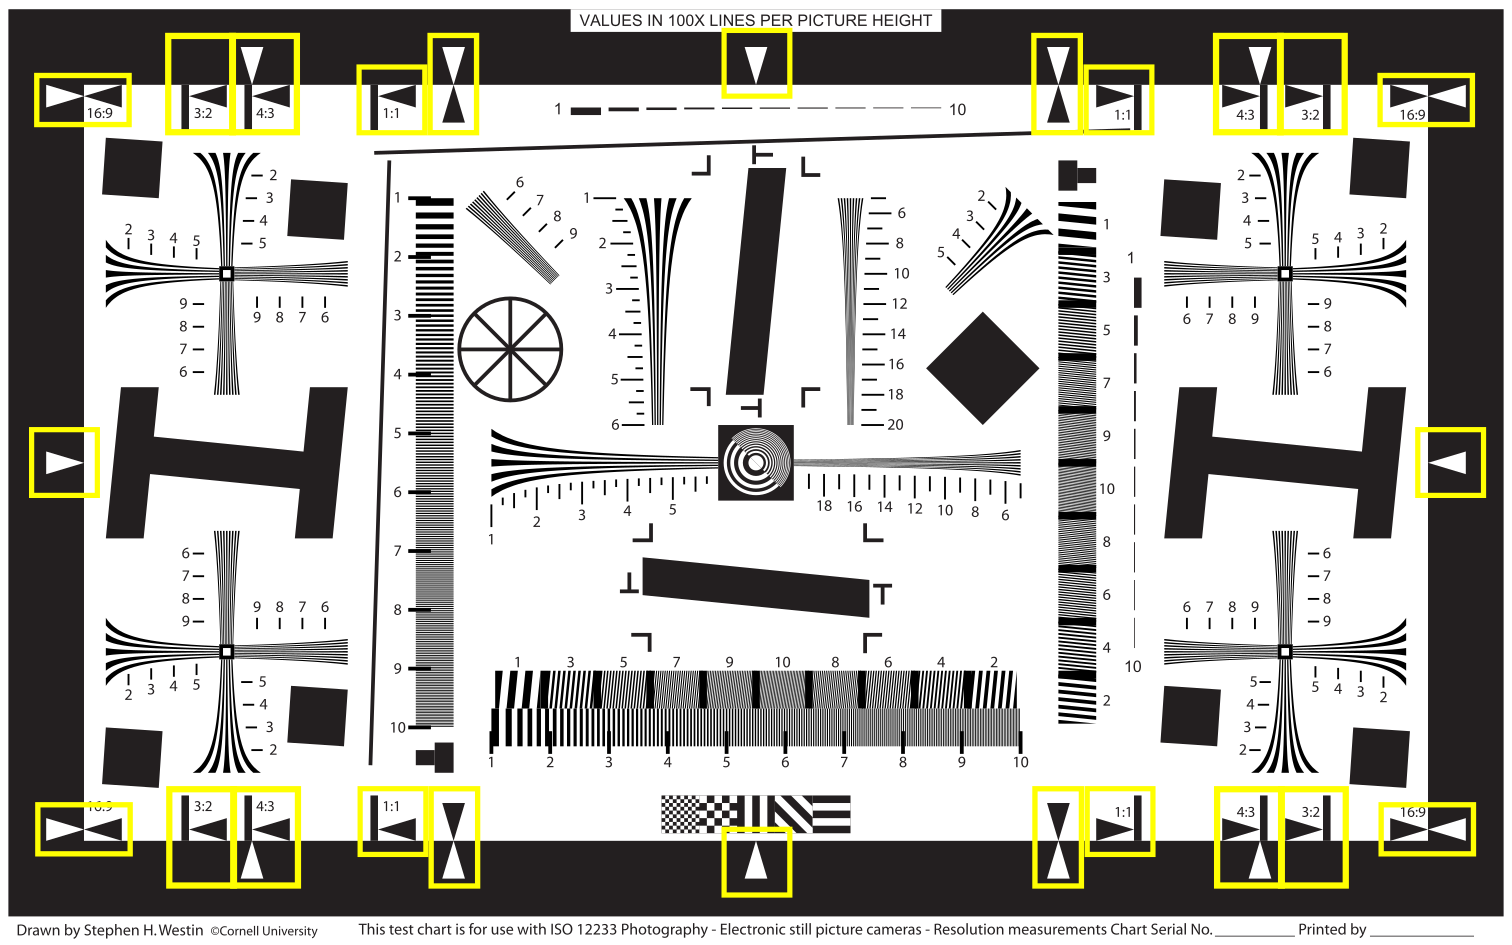
\includegraphics[width=0.8\linewidth]{Figures/C3/ISO_12233-reschart_arrows.png}
        \caption{Standard chart used to measure the spatial frequency response of the optical system. The arrows used for framing and camera alignment are highlighted.}
        \label{fig:iso12233_test_chart_encuadre}
    \end{figure}

    \item The chart is carefully rotated at an angle between $2^\circ$ and $10^\circ$ relative to the sensor’s pixel rows or columns to ensure accuracy in the MTF determination. The chart shown in Figure~\ref{fig:iso12233_test_chart} includes slanted edge patterns that meet this angular requirement.

    \item 50 images of the slanted edge are captured and averaged to reduce temporal noise and improve statistical quality.

    \item 50 dark images are also captured and averaged for sensor non-uniformity correction. This correction is detailed in Section~\ref{subsub:corriente_oscura_espectrometro}.

    \item The slanted edge image is corrected using the previously obtained average dark image.

    \item A specific analysis region is selected within the corrected image, where the slanted edge is clearly distinguishable.

    \item The exact angle of the slanted edge with respect to the sensor rows or columns is determined in order to properly normalize spatial frequency for MTF analysis.

    \item The Edge Spread Function (ESF) is obtained by analyzing pixel intensity values across multiple rows or columns crossing the slanted edge.

    \item To enhance method precision, oversampling is performed by combining multiple rows or columns (at least four) to generate a single, more accurate spatial function.

    \item The ESF is numerically differentiated to generate the Line Spread Function (LSF).

    \item Finally, the Fast Fourier Transform (FFT) is applied to the LSF to obtain the MTF:

    \begin{equation}
        \text{MTF}(f) = \left|\mathcal{F}\{\text{LSF}(x)\}(f)\right|,
    \end{equation}

    where $\mathcal{F}$ denotes the Fourier transform operation and $f$ is the spatial frequency.

    \item The resulting MTF curve is normalized to its maximum value at low frequencies and plotted against spatial frequency for analysis.
\end{enumerate}

MTF processing is performed using the \href{https://imagej.net/ij/plugins/se-mtf/index.html}{SE\_MTF} plugin from \href{https://imagej.net/ij/index.html}{ImageJ}. In this procedure, the image scale is configured in physical units (e.g., lp/mm) based on the actual sensor size and number of photodetectors. Once parameters are configured, the plugin extracts the Edge Spread Function (ESF) from the image edge and, through numerical differentiation, generates the Line Spread Function (LSF). Then, a Fast Fourier Transform (FFT) is applied to the LSF to obtain the Modulation Transfer Function (MTF).

Figure~\ref{fig:plugin_config1} shows the interface for configuring parameters. Based on the Region of Interest (ROI) and pixel size, it is possible to compute the required parameters for plugin configuration.

\begin{figure}[H]
    \centering
    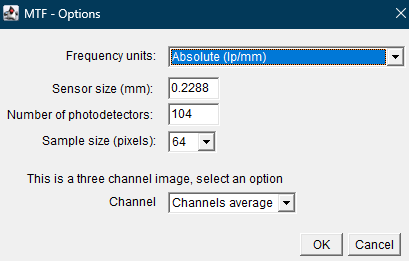
\includegraphics[width=0.6\linewidth]{Figures/C3/imagej_conf.png}
    \caption{Configuration screen of the SE\_MTF plugin in ImageJ. Setup for a Region of Interest of 104 $\times$ 104 pixels and a pixel size of 2.2 $\mu \text{m}$.}
    \label{fig:plugin_config1}
\end{figure}

\subsubsection{Ground–Resolved Distance (GRD) Derived from the MTF}
\label{subsub:grd_from_mtf}

The Modulation Transfer Function provides a frequency–domain representation of the
optical system’s ability to reproduce scene detail.  To translate the laboratory MTF into a
practical “ground” resolution (often called the \emph{ground‑resolved distance}, GRD), the
following procedure is applied\footnote{The workflow follows the recommendations of
ISO~12233 and common practice in remote‑sensing optics
\cite{Boreman2001MTF, Holst2008Electro‑Optical}.}.

\paragraph{1. Identify the cut–off spatial frequency in the image plane.}
From the measured MTF curve, the spatial frequency
$f_{\text{im}}$ (in line‑pairs per millimetre, lp/mm) at which the modulation falls to
30\,\% is chosen as the \emph{cut‑off} frequency:
%
\begin{equation}
    \text{MTF}\bigl(f_{\text{im}}\bigr)=0.30.
    \label{eq:mtf_cutoff}
\end{equation}

\paragraph{2. Convert to object‑space frequency.}
The primary lateral magnification\footnote{For object distances
much larger than the focal length, the primary magnification
$\text{PMAG}$ is well approximated by
$\text{PMAG}= \dfrac{\text{Horizontal Sensor Size}}{\text{FOV}}$;
see Eq.~(\ref{eq:res_0}).} of the lens is
%
\begin{equation}
    \text{PMAG}= \frac{\text{Horizontal Sensor Size}}{\text{FOV}}.
\end{equation}
%
The corresponding frequency in object space is therefore
%
\begin{equation}
    f_{\text{obj}} = \frac{f_{\text{im}}}{\text{PMAG}}
    \quad\left[\frac{\text{lp}}{\text{mm}}\right].
    \label{eq:f_obj}
\end{equation}

\paragraph{3. Compute the linear ground‑resolved distance.}
A line pair consists of one dark and one bright line; hence the minimum
distinguishable physical period on the ground, expressed in micrometres, is
%
\begin{equation}
    \Delta_{\text{ground}} =
    \frac{1}{2\,f_{\text{obj}}}\;\times\;
    \frac{1000\;\mu\text{m}}{1\;\text{mm}}.
    \label{eq:delta_ground}
\end{equation}
%
If a specific flight altitude (working distance) $\text{WD}$ is assumed, the
same result can be expressed directly in metres by multiplying
Eq.~(\ref{eq:delta_ground}) by the scale factor
$\dfrac{\text{WD}}{\text{focal length}}$, yielding the \emph{ground sample
distance} (GSD).

\paragraph{4. Reporting.}
For every lens/sensor pair characterised in
Section~\ref{sec:fov}--\ref{subsub:grd_from_mtf},
Table~\ref{tab:grd_results} lists
$f_{\text{im}}$ at 30\,\% contrast, the computed $f_{\text{obj}}$, and the resulting
$\Delta_{\text{ground}}$ for the three mission altitudes analysed
(50\,m, 1000\,m, and 5000\,m).

\begin{table}[h]
    \centering
    \caption{Ground‑resolved distance (GRD) derived from the 30 \%‑contrast MTF cut‑off. 
             Placeholder numbers are shown; replace them with the values measured for
             each optical system.}
    \label{tab:grd_results}
    \begin{tabularx}{\linewidth}{|l|C|C|C|C|C|}
        \hline
        \rowcolor[HTML]{EFEFEF}
        \textbf{System} & 
        $f_{\text{im}}$ [lp/mm] & 
        $f_{\text{obj}}$ [lp/mm] & 
        GRD @50\,m [cm] & 
        GRD @1000\,m [m] &
        GRD @5000\,m [m] \\
        \hline
        VIS & 85 & 4.3 & 1.2 & 0.23 & 1.15 \\
        NIR & 60 & 2.1 & 2.4 & 0.48 & 2.40 \\
        \hline
    \end{tabularx}
\end{table}





\subsection{Acquisition Settings for VIS and NIR Systems}

The accuracy of resolution and MTF measurements largely depends on the optical system configuration during image capture. In this study, all configurations used for each system were recorded and reported. The following tables summarize the parameters used for the VIS system (visible spectrum camera) and for the NIR system (near-infrared camera):

\begin{longtable}[c]{c|cc|cc}
\hline
\rowcolor[HTML]{EFEFEF} 
\cellcolor[HTML]{EFEFEF} &
  \multicolumn{2}{c|}{\cellcolor[HTML]{EFEFEF}\textbf{FOV}} &
  \multicolumn{2}{c}{\cellcolor[HTML]{EFEFEF}\textbf{MTF}} \\
\rowcolor[HTML]{EFEFEF} 
\multirow{-2}{*}{\cellcolor[HTML]{EFEFEF}\textbf{Parameter}} &
  \textbf{VIS} &
  \textbf{NIR} &
  \textbf{VIS} &
  \textbf{NIR} \\ \hline
\endfirsthead
%
\endhead
%
\hline
\endfoot
%
\endlastfoot
%
\textbf{ExposureTime (ms)}  & 18264.15 & 498463.3 & 2636.135 & 47487.15 \\
\rowcolor[HTML]{EFEFEF} 
\textbf{Gain}               & 0.0      & 24.1     & 0.0      & 0.0      \\
\textbf{Height (pixels)}    & 1944     & 1944     & 104      & 104      \\
\rowcolor[HTML]{EFEFEF} 
\textbf{Width (pixels)}     & 2592     & 2592     & 104      & 104      \\
\textbf{OffsetX}            & 0        & 0        & 1230     & 1200     \\
\rowcolor[HTML]{EFEFEF} 
\textbf{OffsetY}            & 0        & 0        & 920      & 900      \\
\textbf{Gamma}              & 1.0      & 1.0      & 1.0      & 1.0      \\
\rowcolor[HTML]{EFEFEF} 
\textbf{Hue}                & 0.0      & --       & 0.0      & --       \\
\textbf{BalanceRatio\_Red}  & 1.307617 & --       & 1.289063 & --       \\
\rowcolor[HTML]{EFEFEF} 
\textbf{BalanceRatio\_Blue} & 1.957031 & --       & 1.979004 & --       \\ \hline
\caption{Acquisition Configuration for MTF and FOV Experiments (VIS and NIR)}
\label{tab:tab:fov_mtf}\\
\end{longtable}

Below is a brief description of each parameter used in the configuration:

\begin{itemize}
    \item \textbf{ExposureTime:} Exposure time in milliseconds, determining how long the sensor collects light. Longer exposures increase the captured light but may cause saturation if not properly adjusted.

    \item \textbf{Gain:} Sensor gain factor, amplifying the generated electrical signal. A high gain may increase noise; hence, it is set to 0.0 to avoid unwanted amplification.

    \item \textbf{Gamma:} Gamma correction applied to the image, adjusting the linearity of the light response. A value of 1.0 ensures a linear response.

    \item \textbf{Height (pixels):} Image height in pixels. This parameter defines the vertical resolution and the area of interest.

    \item \textbf{Width (pixels):} Image width in pixels. Together with height, it defines the spatial resolution of the sensor.

    \item \textbf{OffsetX and OffsetY:} Horizontal (OffsetX) and vertical (OffsetY) displacements of the capture area over the sensor. These values help center or adjust the region of interest according to the position of the object or test chart.

    \item \textbf{Hue:} Hue adjustment in the image, used only in color cameras (VIS system). A value of 0.0 means no tonal adjustment is applied.

    \item \textbf{BalanceRatio\_Red and BalanceRatio\_Blue:} White balance ratios for the red and blue channels in color cameras. These coefficients are used to match the responses of each channel and ensure proper white balance. In this study, they were manually adjusted to overlap the peaks of the bright zone in the RGB histograms.
\end{itemize}

These settings are defined to ensure maximum signal without saturation and to avoid clipping in bright and dark areas, guaranteeing that the slanted-edge image is captured under controlled conditions. These parameters are recorded to allow for study replication and for detailed analysis of the optical system response under both low- and high-intensity conditions.

\section{Spectral Characterization of Multispectral Cameras}

Spectral characterization is a fundamental process for color calibration and accurate spectral estimation in multispectral cameras. This process is particularly relevant in applications such as remote sensing, precision agriculture, and environmental analysis, where precision in detecting different wavelengths determines the quality of the obtained data. For this characterization, two main calibration methods using a monochromator were employed: joint calibration of the entire system and separate calibration of its components.

\subsection{Experimental Procedure in the Laboratory}
\label{sec:procedimiento_experimental_laboratorio}

This section details the laboratory procedure used for the spectral response characterization of various optical systems. The methodology includes the selection of the illumination source, validation of its spectrum, beam collimation, dark current correction of the minispectrometer, use of a set of filters and acrylic sheets, selection and combination of said filters, determination of the central wavelength, and measurement of optical power, followed by image capture with the optical system under test.

\subsubsection{Selection and Validation of the Illumination Source}
\label{subsub:fuente_validacion}

A tungsten lamp from ThorLabs, model OSL-2~\cite{OSL2-Manual}, was selected as the main illumination source. This type of lamp emits radiation over a broad range, approximately from 400 nm to 1600 nm, which is suitable for covering both the visible and part of the near-infrared spectrum.

To ensure the spectral distribution of the lamp matched expectations, a minispectrometer from Newport (reference pending) was used to measure its output spectrum. Figure~\ref{fig:lampara_tungsteno_espectro} shows an example of the measured spectral signal, expressed in \textit{counts}, which is the standard output format of such spectrometers. These counts represent the relative intensity recorded by the spectrometer's sensor, but do not constitute an absolute radiometric quantity. Therefore, to obtain a fully calibrated measurement, these counts must be related to the optical power measured by an independent power meter.

\begin{figure}[h!]
    \centering
    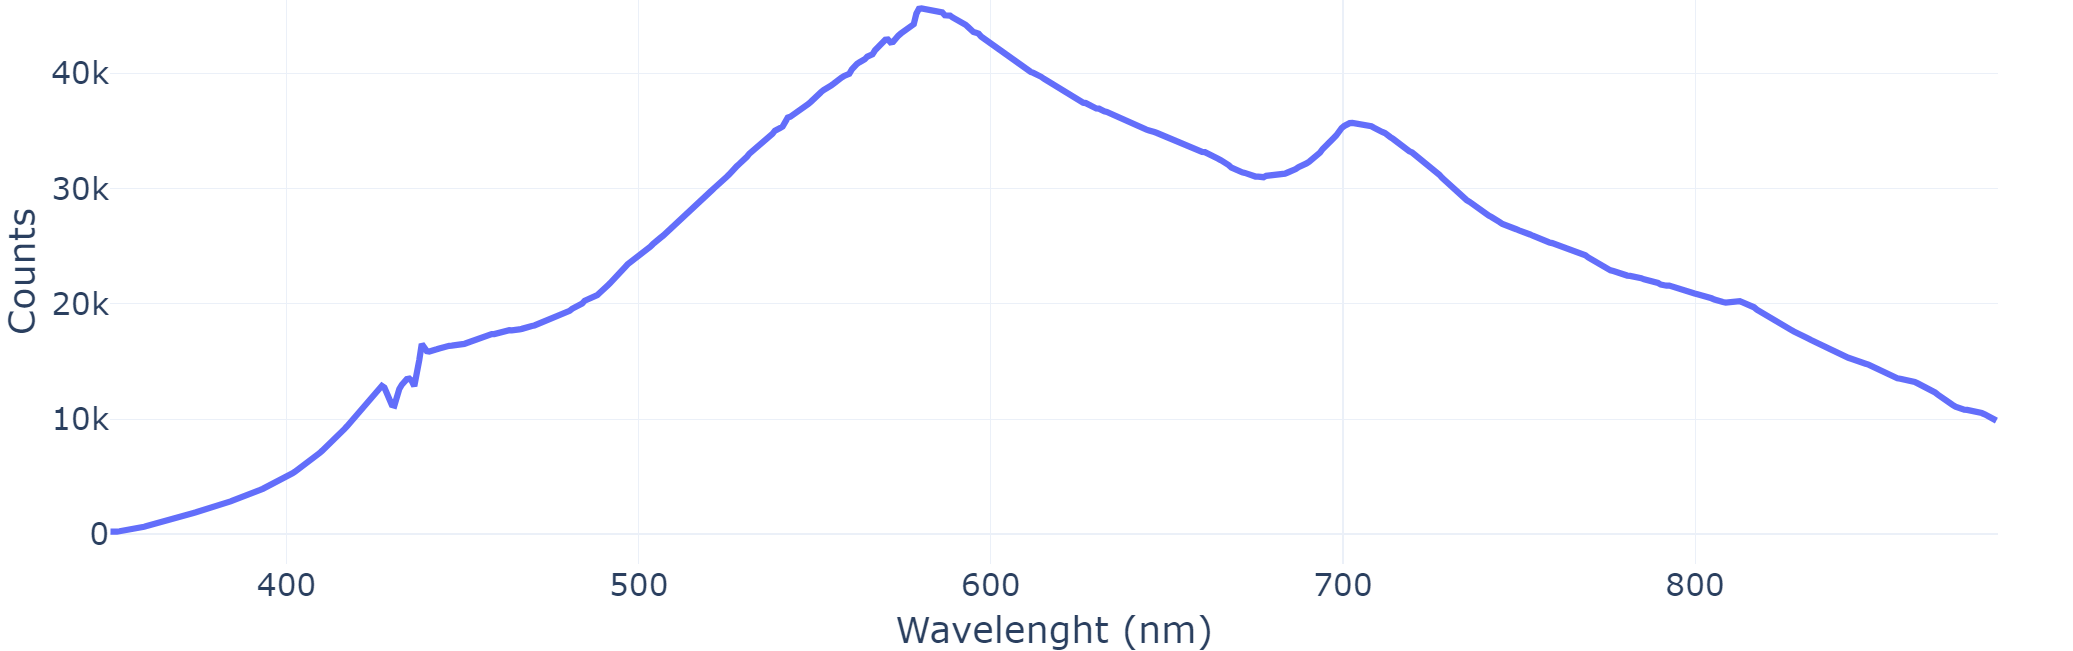
\includegraphics[width=1\textwidth]{Figures/C3/tunsteno.png}
    \caption{Example of the measured spectrum of the tungsten lamp (OSL-2) using the minispectrometer. The vertical axis is expressed in counts, which depend on the intrinsic response of the spectrometer.}
    \label{fig:lampara_tungsteno_espectro}
\end{figure}

\subsubsection{Setup and Collimation of the Illumination Beam}
\label{subsub:montaje_colimacion}

The tungsten lamp mentioned includes a fiber optic coupling that allows directing the light toward various optical elements. The wavefront emerging from the fiber optic is \emph{divergent}, so the optical power decreases significantly as the distance between the fiber output and the measurement plane increases. To work under controlled conditions and optimize power utilization, the light beam was \textbf{collimated} by mounting the fiber in a one-inch diameter lens tube.

\begin{enumerate}
    \item \textbf{Selection of the collimating lens:} A plano-convex lens with a focal length of $25$\,mm was selected. Although a longer focal length would reduce divergence, in practice, using lenses with longer focal lengths limits the effective light collection area (especially when the source is not a point source), thus decreasing the total power available in the collimated beam. A 25\,mm lens provides greater light collection, albeit at the cost of slightly more divergence.
    
    \item \textbf{Collimation method:}
    \begin{itemize}
        \item Traditionally, collimation is achieved by measuring the spot size at various distances along the optical axis and adjusting the lens position to find the point where the beam shows a more constant diameter (or minimum divergence) along its propagation. However, this method was not used in this work due to:
        \begin{enumerate}
            \item The lens used is spherical, and the beam coming from the fiber (an extended source) causes noticeable divergence, making it difficult to pinpoint the collimation position solely by observing the spot.
            \item The main goal is to ensure maximum usable optical power at the measurement plane, making it inefficient to characterize beam uniformity based only on spot size.
        \end{enumerate}
        
        \item Instead, an optical power meter is placed at a fixed distance from the collimating lens (see Figure~\ref{fig:montaje_colimacion}).
        \item A 4\,nm bandwidth filter centered at 633\,nm is placed in the optical path to isolate a specific spectral range and reduce dispersive effects.
        \item The distance between the fiber and the lens is varied around the nominal focal length (25\,mm), \emph{searching for the maximum optical power} measured at the detector. This point indicates minimum beam divergence near the measurement plane and maximum power collection.
    \end{itemize}
    
    \item \textbf{Final positioning:} Once the position that maximizes the detected power is found, the positions of the fiber and the lens are mechanically fixed. Additionally, the distance between the lens and the power meter is kept constant for subsequent measurements, ensuring consistent illumination conditions.
\end{enumerate}

\begin{figure}[h!]
    \centering
    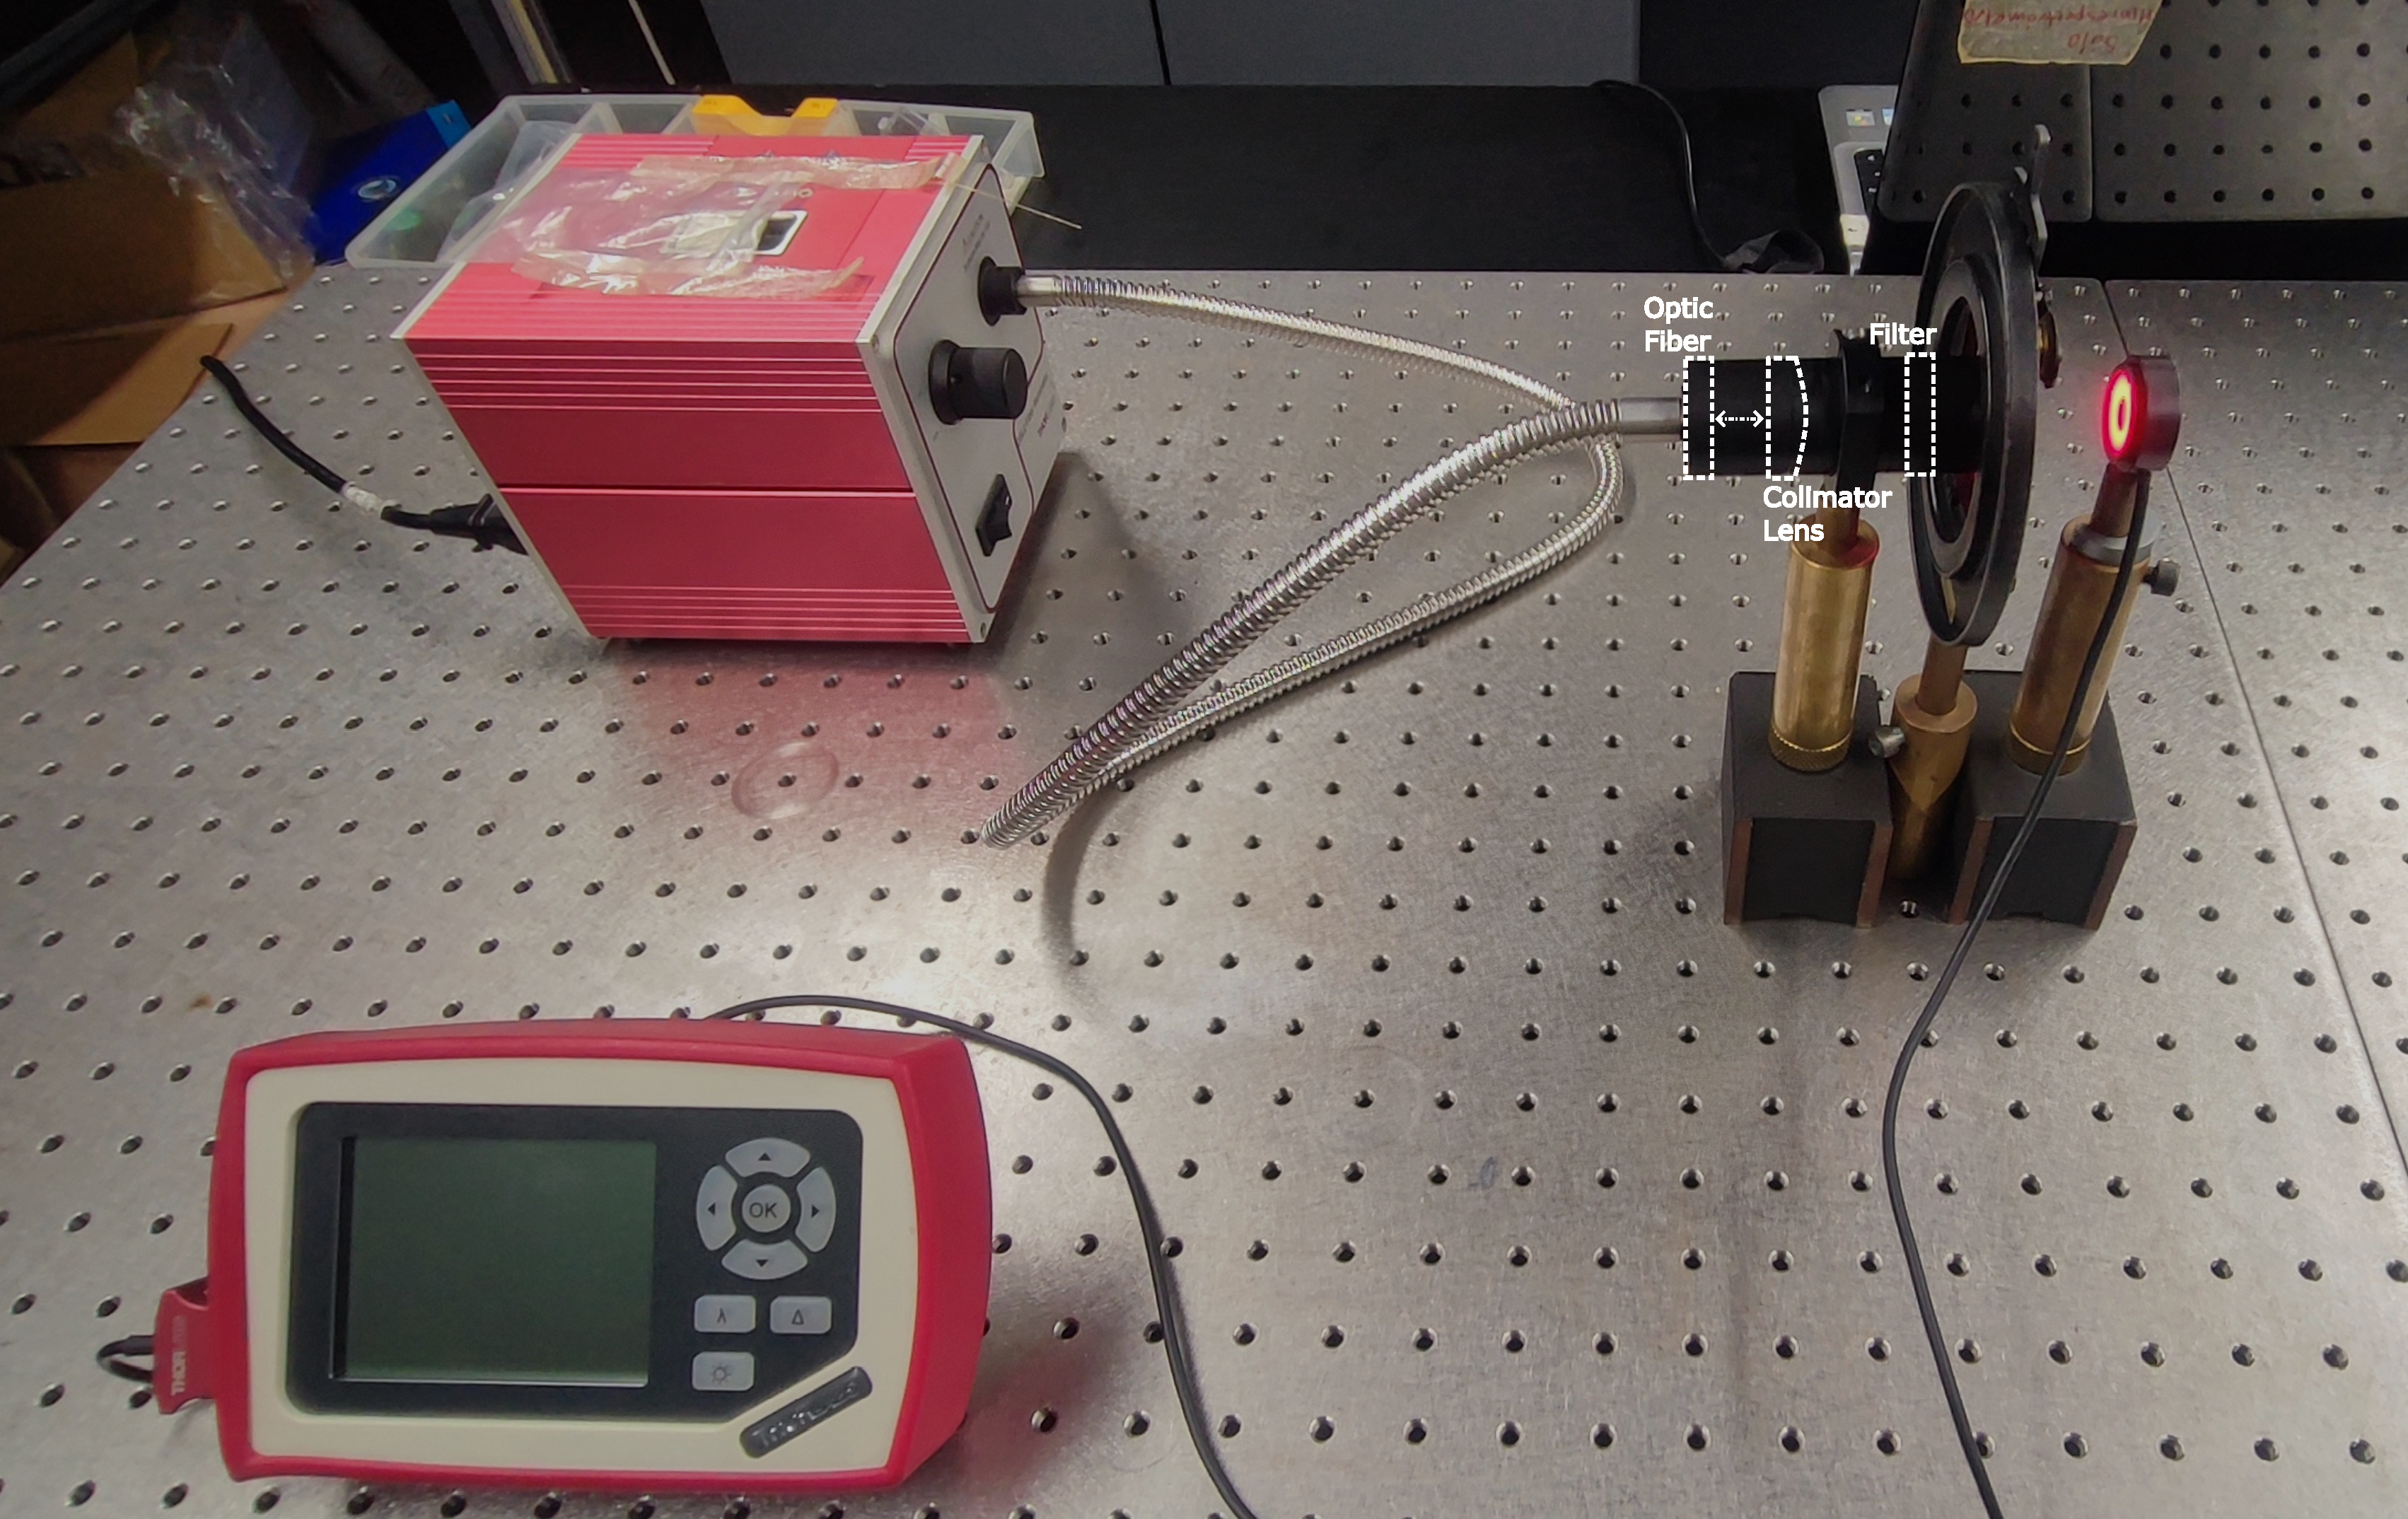
\includegraphics[trim=30mm 0mm 40mm 25mm, clip, width=0.9\textwidth]{Figures/C3/colimacion.pdf}
    \caption{Setup for collimating the beam of the tungsten lamp with fiber optics. The adjustment of the distance between the fiber and the plano-convex lens aims to maximize the optical power measured by the detector.}
    \label{fig:montaje_colimacion}
\end{figure}

\subsubsection{Dark Current Correction in the Minispectrometer}
\label{subsub:corriente_oscura_espectrometro}

The minispectrometer used to validate the light source spectrum and measure the transmissions of different filters records a base signal even without illumination, known as \emph{dark current} or \emph{electronic noise}. To improve the accuracy of spectral measurements, the following procedure was applied:

\begin{itemize}
    \item A reference measurement was taken under \textbf{total absence of light} (fiber and input blocked). This signal is denoted by \(\mathbf{D}\) and corresponds to the electronic noise level.
    
    \item For any measured spectrum \(\mathbf{S}\) (e.g., the spectrum of the tungsten lamp or a specific filter), correction is applied by subtracting \(\mathbf{D}\):
    \[
        \mathbf{S}_{\text{corr}} \;=\; \mathbf{S} \;-\; \mathbf{D}.
    \]
\end{itemize}

This attenuates the offset due to readout noise and provides a more reliable reading of the spectral distribution in \emph{counts}.

\subsubsection{Set of Filters and Acrylic Sheets}
\label{subsub:filtros_laminas}

To discretize or modify the spectral distribution of the tungsten lamp, the following elements were used:

\begin{itemize}
    \item \textbf{Nine high-quality optical filters} mountable in one-inch tubes. These filters are numbered from 0 to 6, with two additional filters labeled 532 and 633 (corresponding to their central wavelengths).
    
    \item \textbf{Eight acrylic sheets} of different colors, each 2\,x\,2\,inches, mountable in an optical slide holder.
\end{itemize}

Figure~\ref{fig:laminas_filtros} shows the filters and acrylic sheets with their respective labels. The transmitted spectrum of each element was measured (using the tungsten lamp as the illumination source) with the minispectrometer. These measurements were corrected for dark current as described in Section~\ref{subsub:corriente_oscura_espectrometro}.

\begin{figure}[h!]
    \centering
    \begin{subfigure}{\textwidth}
        \centering
        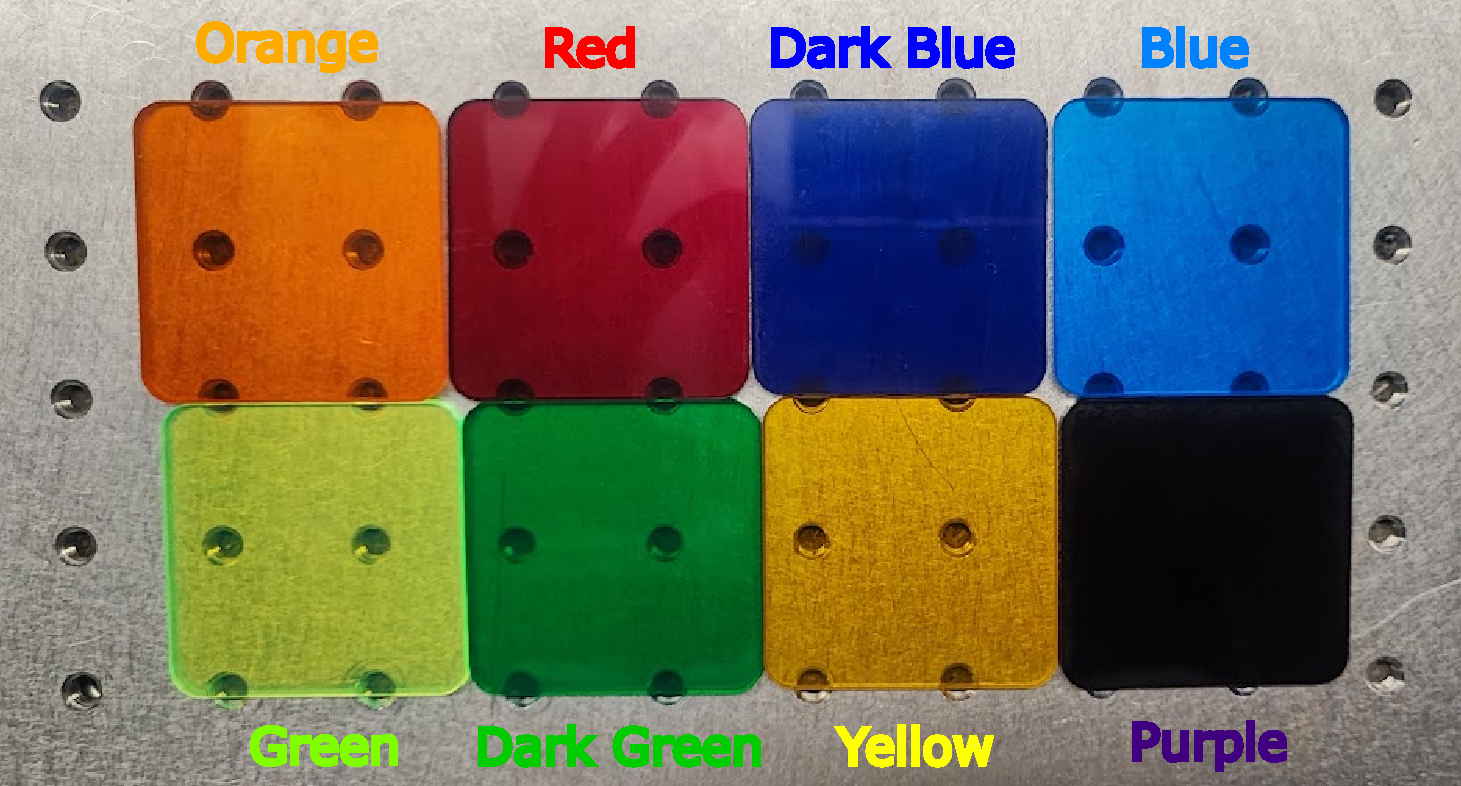
\includegraphics[width=0.8\textwidth]{Figures/C3/laminas.pdf}
        \caption{Set of acrylic sheets used. Each is individually labeled based on its apparent color.}
        \label{fig:laminas}
    \end{subfigure}
    \vspace{1em}
    \begin{subfigure}{\textwidth}
        \centering
        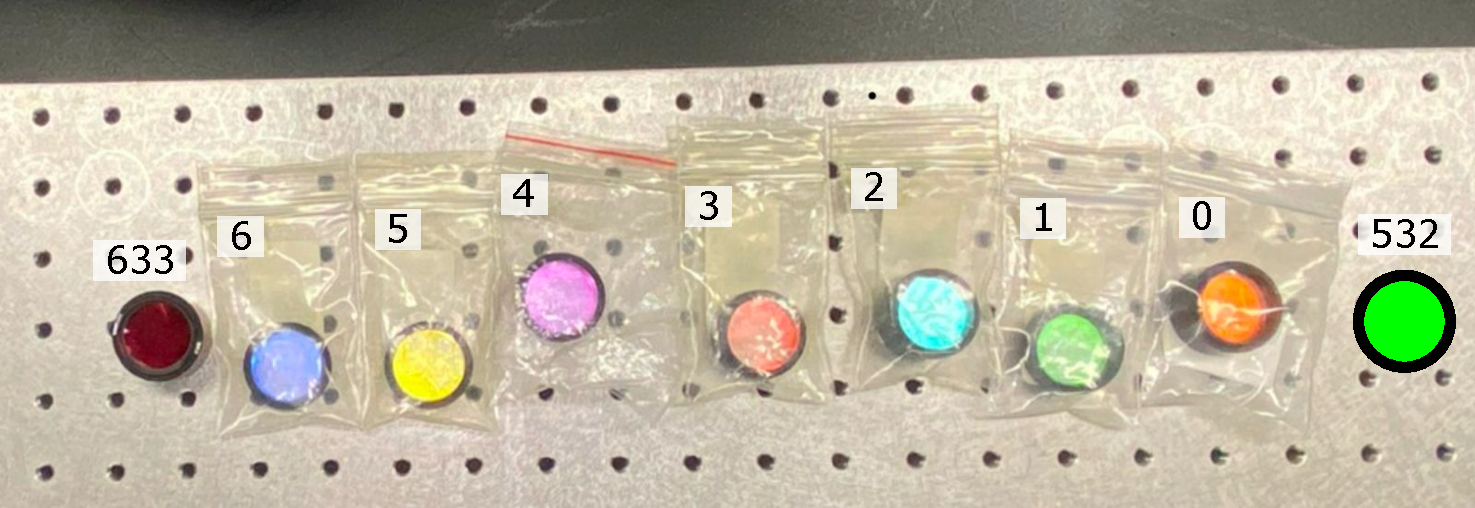
\includegraphics[width=0.8\textwidth]{Figures/C3/filtros.pdf}
        \caption{Set of filters used. Filters are numbered 0 to 6, with two additional filters labeled 532 and 633.}
        \label{fig:filtros}
    \end{subfigure}
    \caption{Acrylic sheets and filters used in the experiment.}
    \label{fig:laminas_filtros}
\end{figure}

\subsubsection{Measurement of Transmission Spectra}
\label{subsub:medicion_transmision}

The transmission spectra of each filter and acrylic sheet are measured to determine their effective spectral transmission. Figure~\ref{fig:montaje_spec} shows the optical setup used to measure the transmission spectrum.

\begin{figure}[h!]
    \centering
    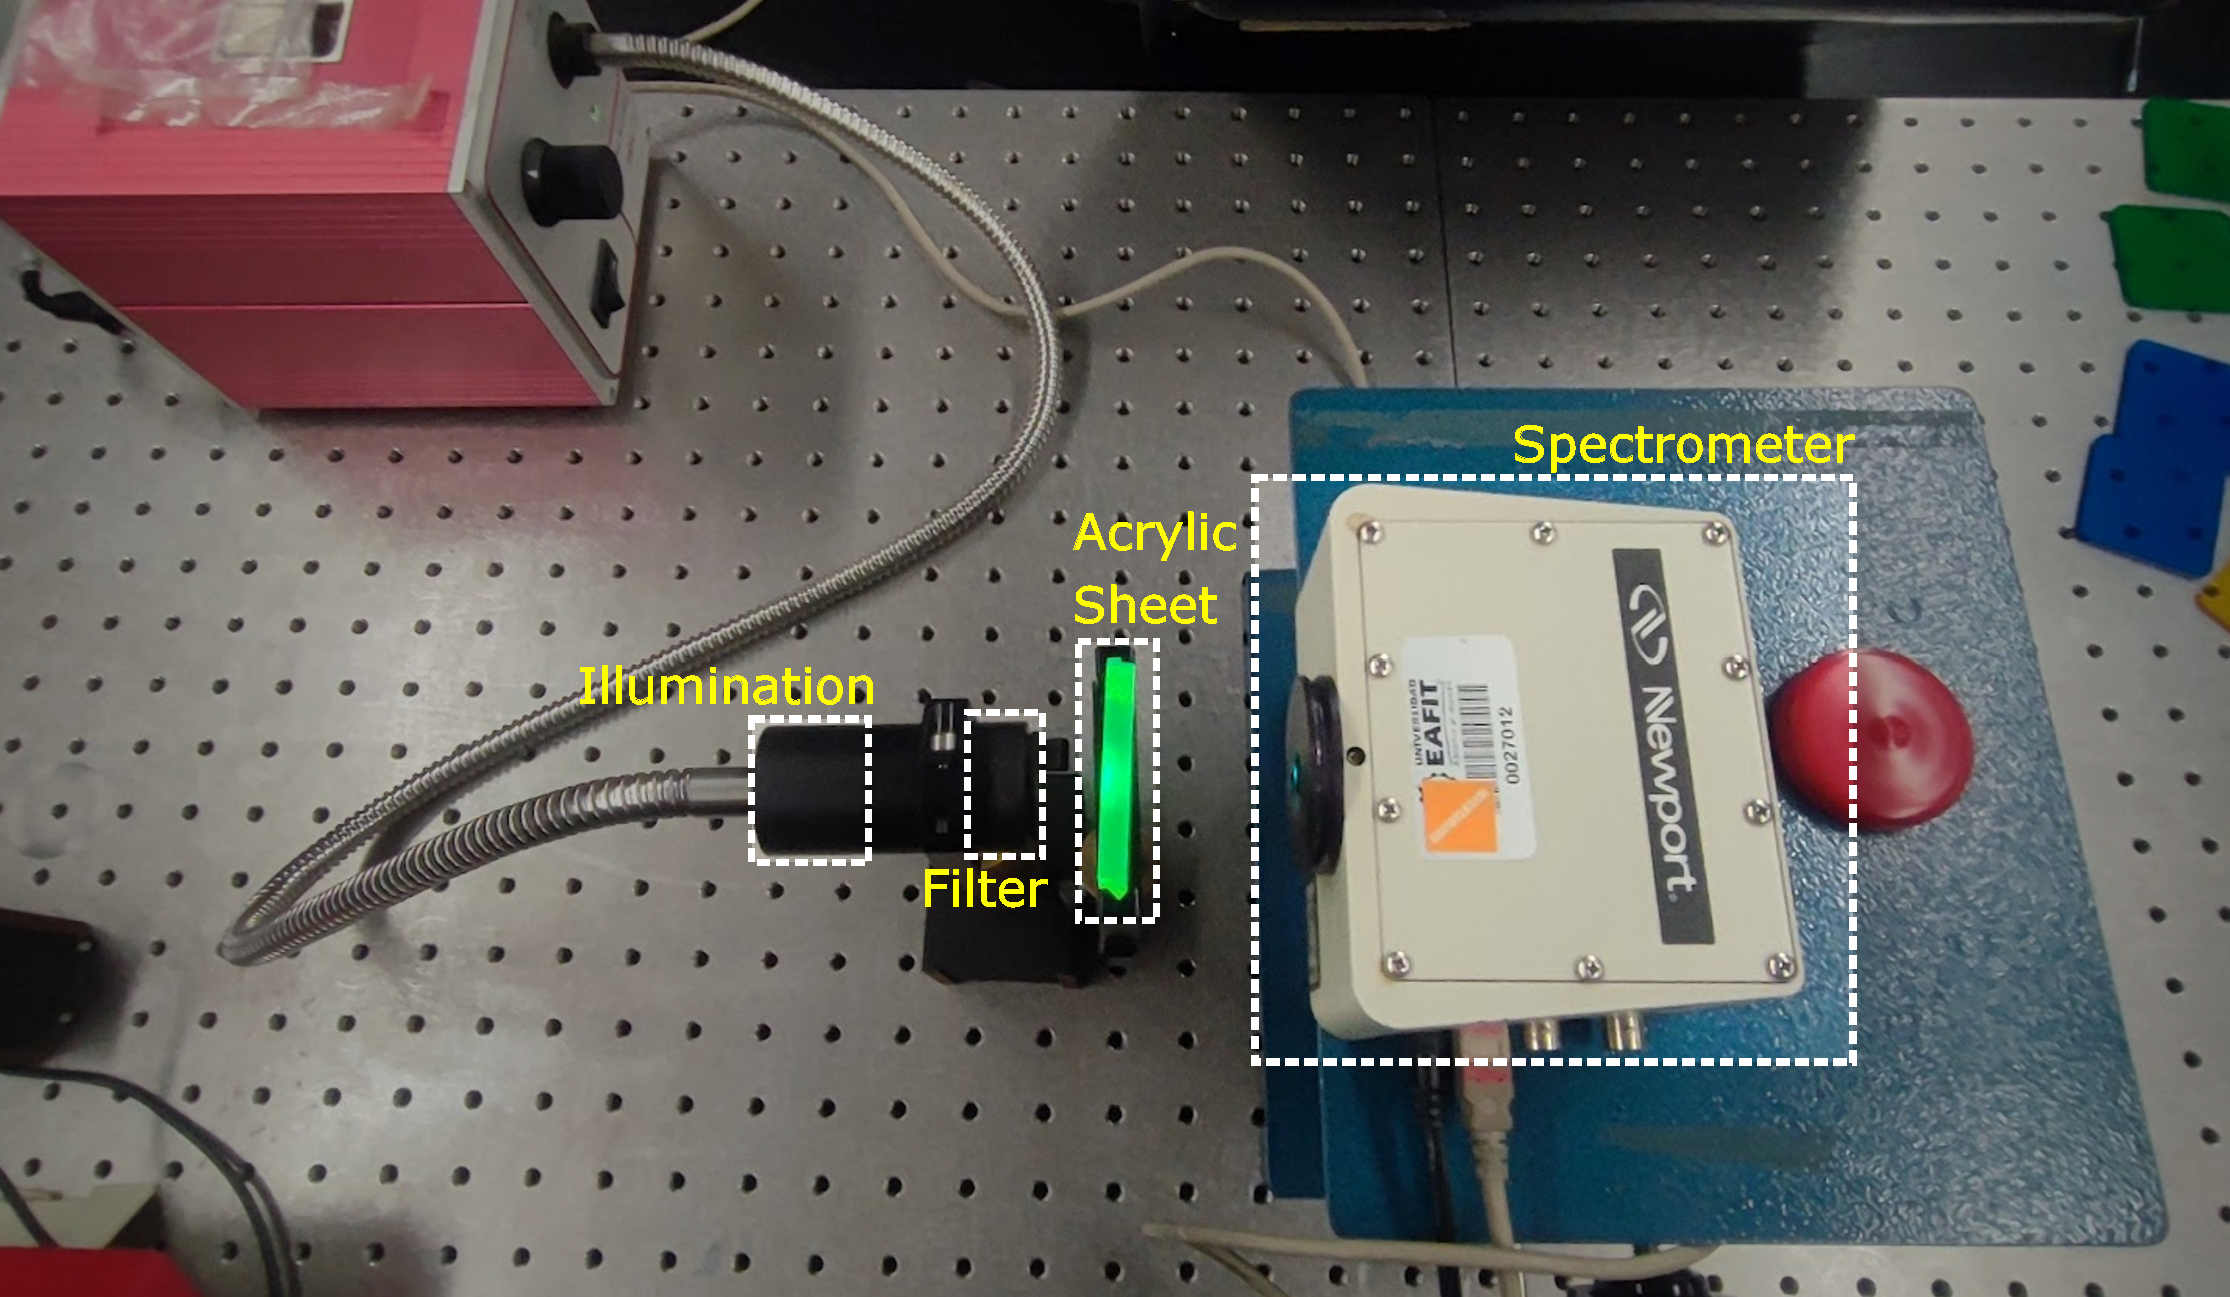
\includegraphics[trim=30mm 0mm 40mm 25mm, clip, width=0.9\textwidth]{Figures/C3/montaje_spec.pdf}
    \caption{Setup for measuring the transmission spectrum of filters and acrylic sheets.}
    \label{fig:montaje_spec}
\end{figure}

\begin{itemize}
    \item For the \textbf{illumination}, the base spectrum \(\mathbf{I}\) is obtained (dark-current corrected).
    \item For each \textbf{filter} or \textbf{sheet}, the transmitted spectrum \(\mathbf{T}_j\) is measured, also corrected for dark current.
\end{itemize}

The recorded spectra are shown in Figure~\ref{fig:espectros_combinados}. Then, the dimensionless relative spectral response for each element is calculated by dividing \(\mathbf{T}_j\) by \(\mathbf{I}\). The justification lies in the fact that, in linear systems, the transmission is modeled as a multiplication of the source spectrum by the spectral transfer function of the element (filter or sheet):

\[
    \mathbf{T}_j \;=\; \mathbf{I} \;\times\; \beta_j(\lambda),
\]
\[
    \frac{\mathbf{T}_j}{\mathbf{I}} \;=\; \beta_j(\lambda).
\]

Thus, the curve \(\beta_j(\lambda)\) represents the \textbf{effective spectral transmittance} of the filter or sheet (see Figure~\ref{ig:filtros_laminas_espectros_relativos}).

\begin{figure}[h!]
    \centering
    \begin{subfigure}{\textwidth}
        \centering
        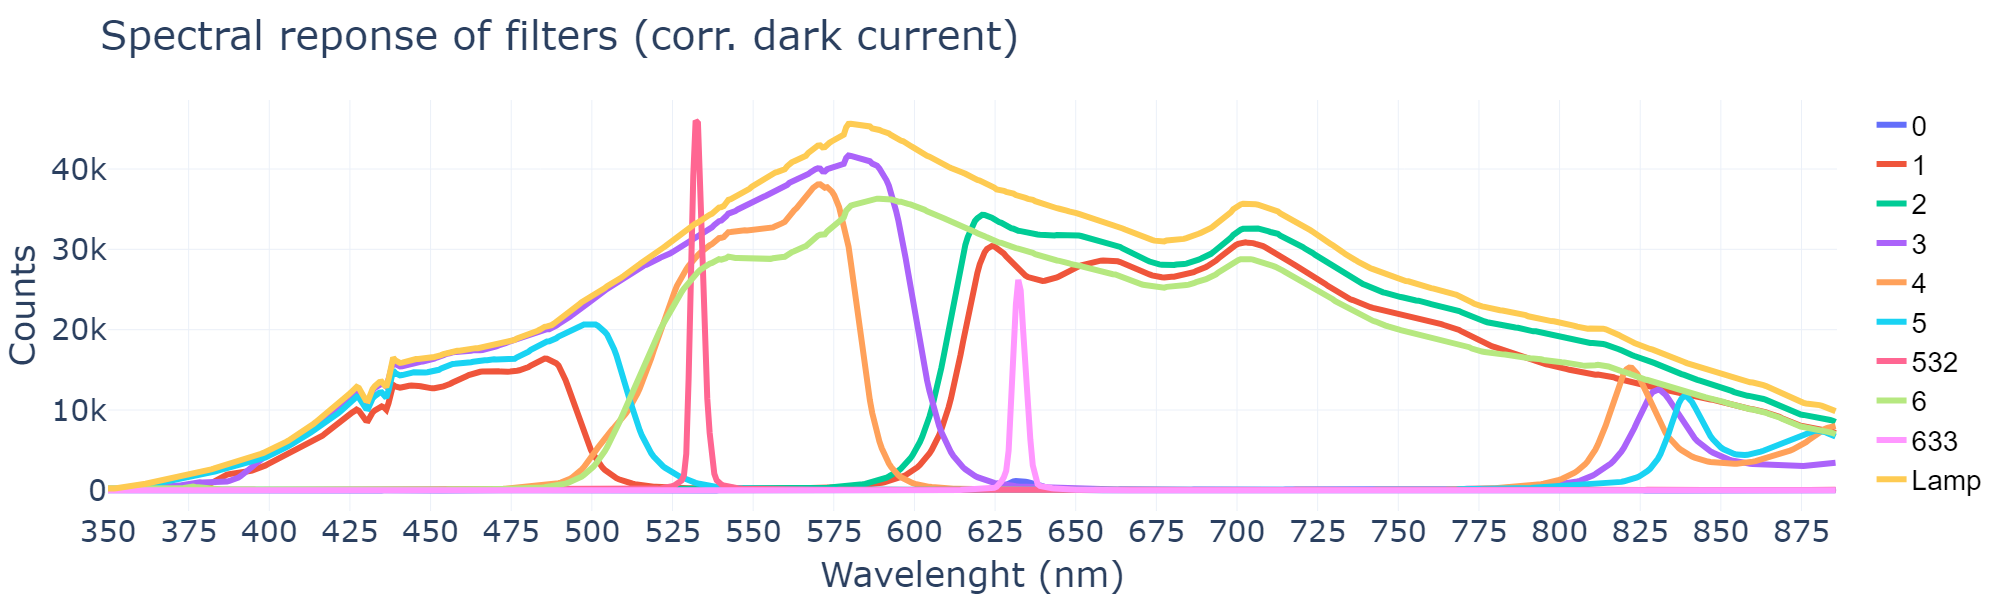
\includegraphics[trim=0mm 0mm 0mm 25mm, clip, width=0.9\textwidth]{Figures/C3/filtros_spec.png}
        \caption{Filters.}
        \label{fig:filtros_espectros}
    \end{subfigure}
    \vspace{1em}
    \begin{subfigure}{\textwidth}
        \centering
        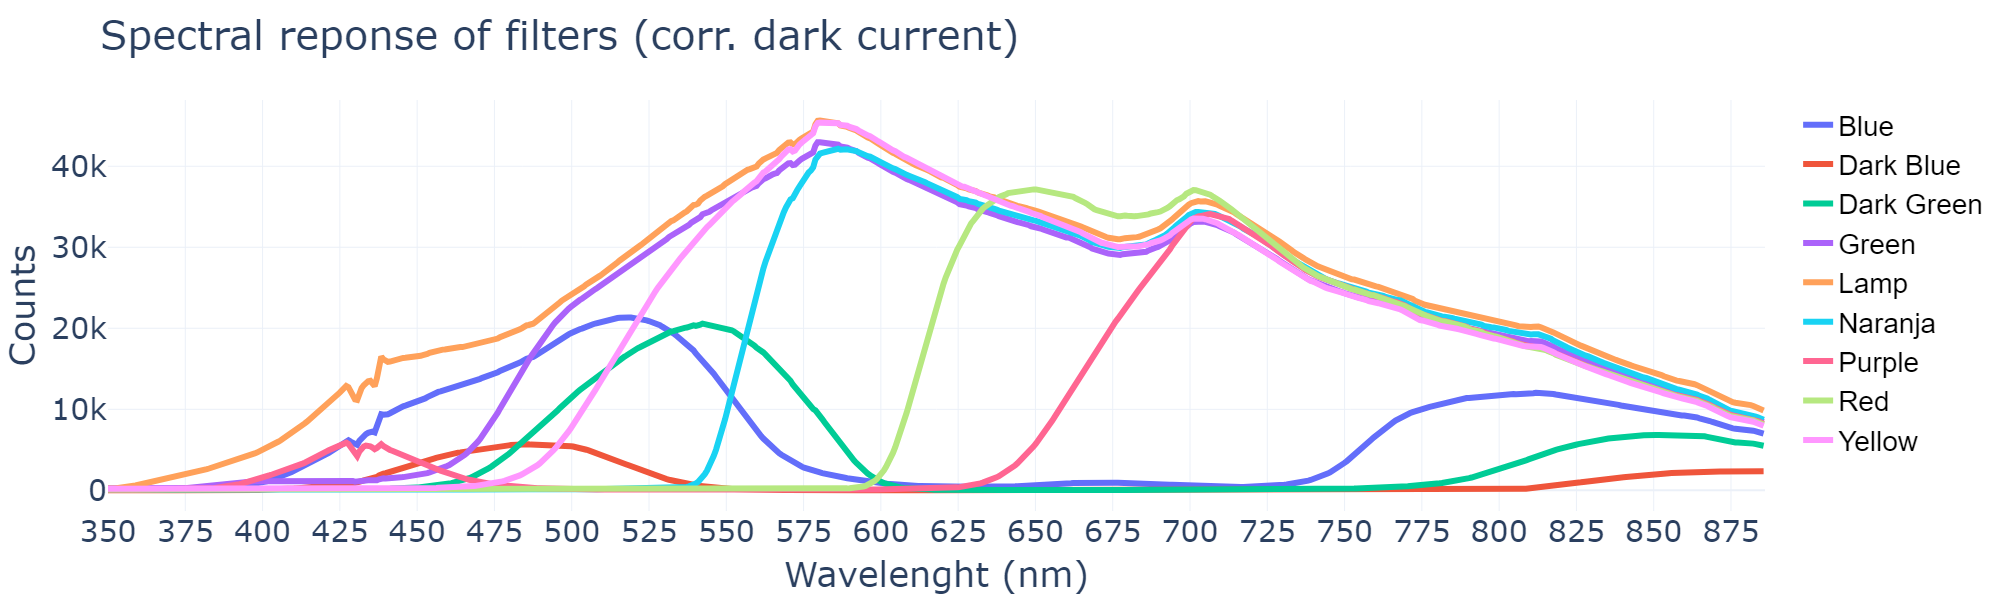
\includegraphics[trim=0mm 0mm 0mm 25mm, clip, width=0.9\textwidth]{Figures/C3/laminas_spec.png}
        \caption{Acrylic plates.}
        \label{fig:laminas_espectros}
    \end{subfigure}
    \caption{Measured spectra (in counts) of tungsten light transmitted through various filters (A) and acrylic plates (B). The vertical axis shows the relative intensity recorded by the minispectrometer in counts.}
    \label{fig:espectros_combinados}
\end{figure}

\begin{figure}[h!]
    \centering
    \begin{subfigure}{\textwidth}
        \centering
        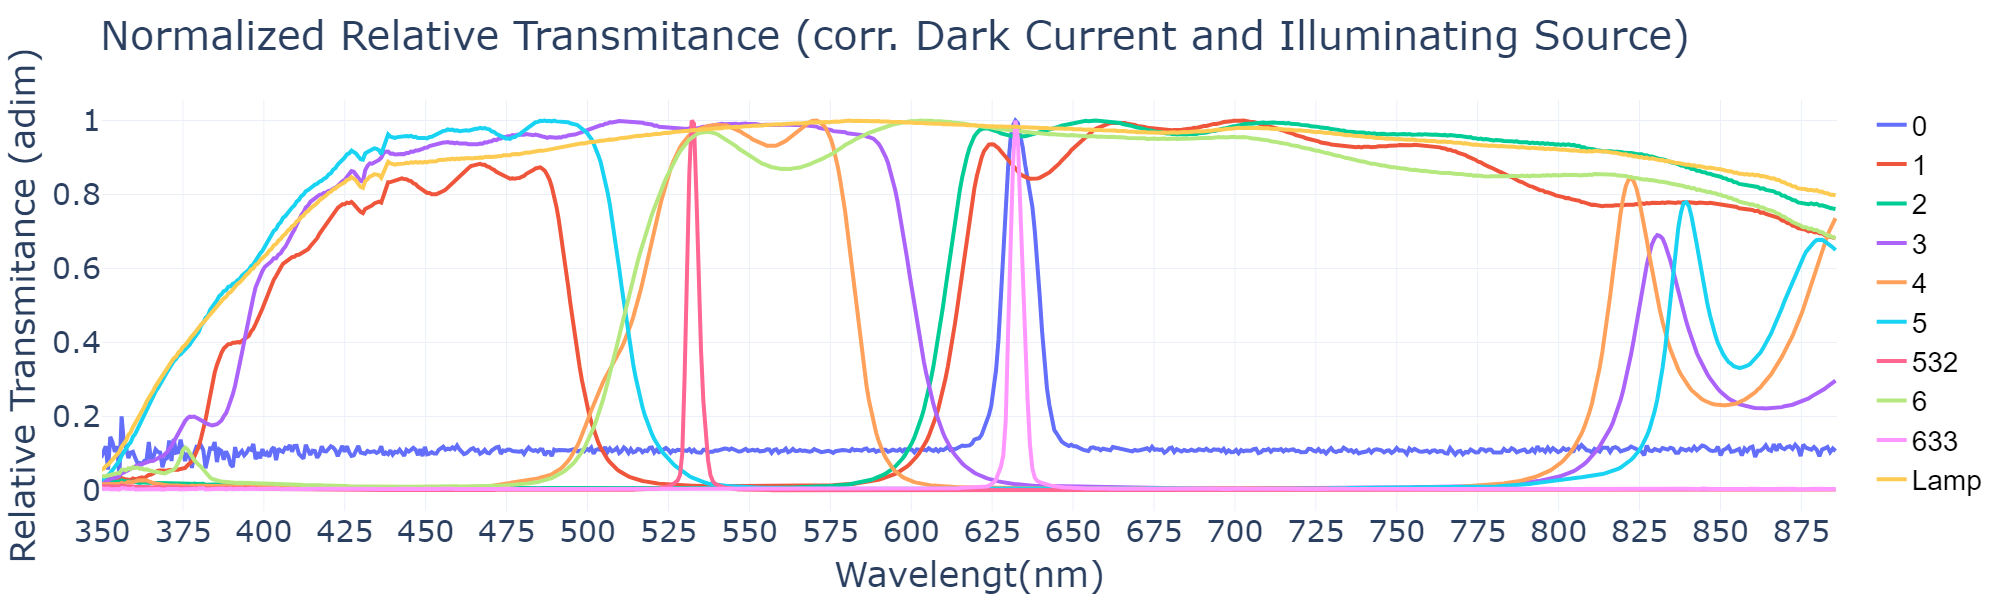
\includegraphics[trim=0mm 0mm 0mm 25mm, clip, width=0.9\textwidth]{Figures/C3/filtros_respuestaspec.png}
        \caption{Filters.}
        \label{fig:filtros_espectros}
    \end{subfigure}
    \vspace{1em}
    \begin{subfigure}{\textwidth}
        \centering
        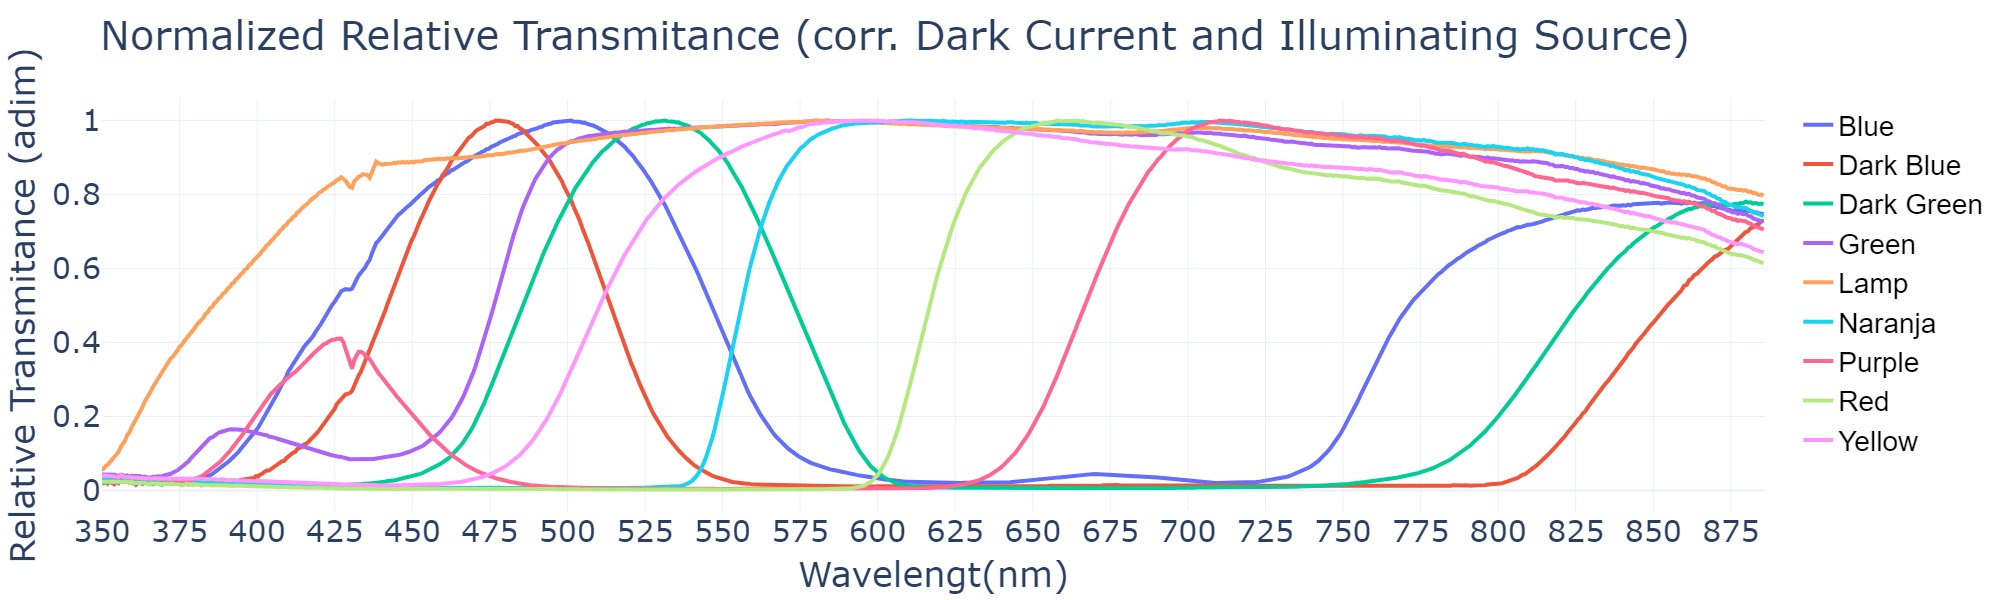
\includegraphics[trim=0mm 0mm 0mm 25mm, clip, width=0.9\textwidth]{Figures/C3/laminas_respuestaspec.png}
        \caption{Acrylic plates.}
        \label{fig:laminas_espectros}
    \end{subfigure}
    \caption{Normalized dimensionless spectral response (transmittance) obtained by dividing each filtered spectrum by the tungsten lamp spectrum.}
    \label{ig:filtros_laminas_espectros_relativos}
\end{figure}

\subsubsection{Generación y selección de combinaciones de filtros}
\label{subsub:combinaciones_filtros}

\subsubsection{Generation and Selection of Filter Combinations}
\label{subsub:combinaciones_filtros}

Given that the filters have relatively wide bandwidths (many exceeding 100 nm), this work evaluates the possibility of combining up to three filters to obtain more selective transmission curves. A \texttt{Python} script is developed that:

\begin{enumerate}
    \item Lists all possible combinations of:
    \begin{itemize}
        \item Individual filters and/or acrylic sheets,
        \item Pairs of filters/sheets,
        \item Triplets of filters/sheets.
    \end{itemize}
    \item For each combination, calculates the \emph{composite transmission curve} \(\beta_{\text{comp}}(\lambda)\), which is the \textbf{product} of the individual transmissions as a function of wavelength.
    \item Generates a total of 987 combinations (including single, double, and triple combinations).
\end{enumerate}

\paragraph{Ideal Transmission Curves.}
To guide the selection process, 10 target curves are defined, modeled as Gaussian functions with a standard deviation of 3\,nm:

\begin{itemize}
    \item Seven curves centered in the visible spectrum: 400, 450, 500, 550, 600, 650, and 700\,nm.
    \item Three curves for the near-infrared (NIR): 825, 850, and 875\,nm.
\end{itemize}

Each \(\beta_{\text{ideal}}(\lambda)\) adopts the form:
\[
\beta_{\text{ideal}}(\lambda) \;=\; \exp\!\Big[-\tfrac{(\lambda - \lambda_0)^2}{2 \,\sigma^2}\Big],
\]
where \(\lambda_0\) is the central wavelength and \(\sigma=3\) nm.  
Figure~\ref{fig:curvas_ideales} illustrates the ideal profiles used.

\begin{figure}[h!]
    \centering
    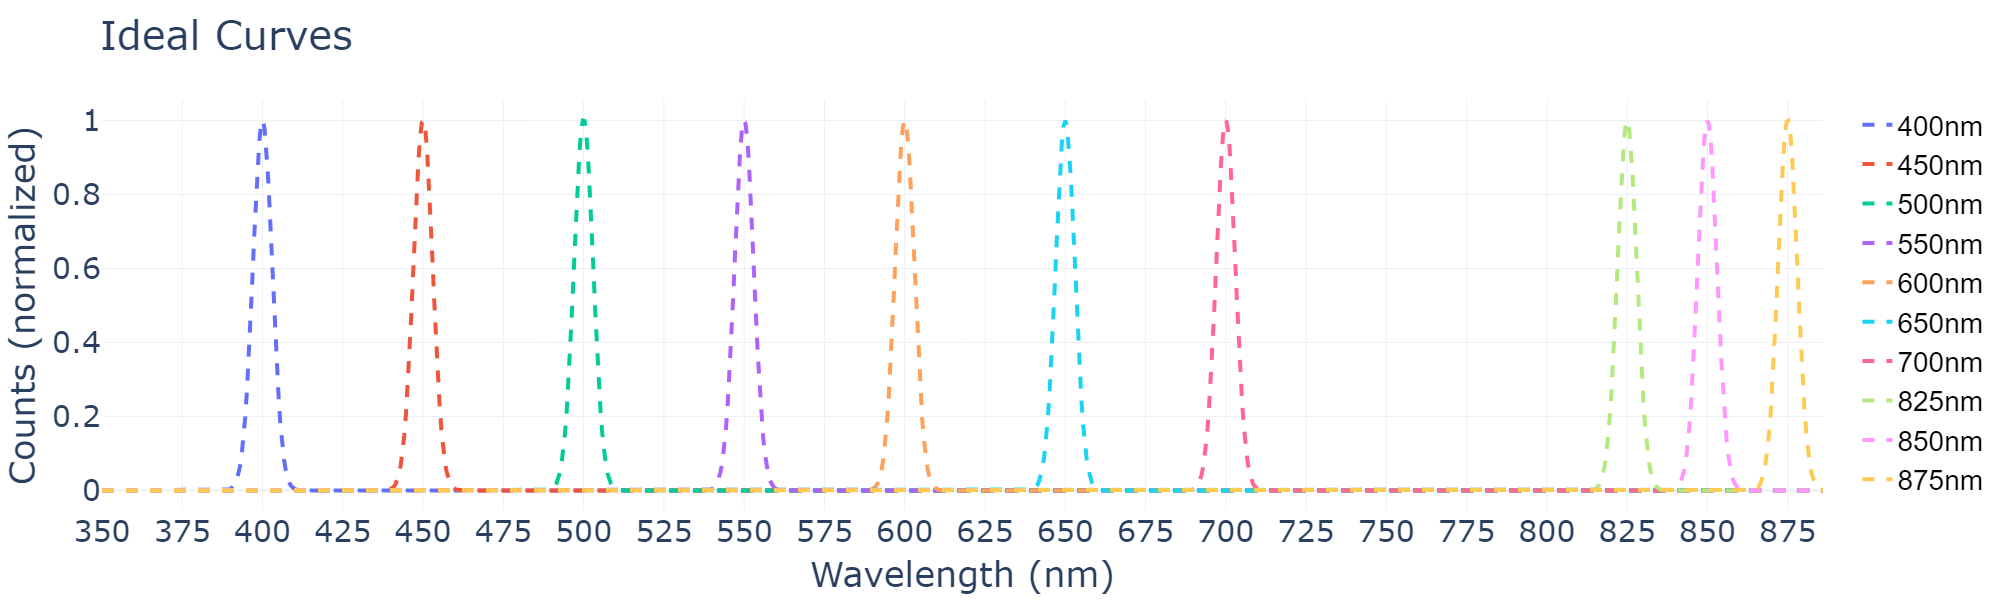
\includegraphics[trim=0mm 0mm 0mm 25mm, clip, width=1\textwidth]{Figures/C3/ideal_spec.png}
    \caption{Ideal transmission curves for selecting filter combinations. This example shows 10 Gaussians centered at 400, 450, 500, 550, 600, 650, 700, 825, 850, and 875 nm, respectively.}
    \label{fig:curvas_ideales}
\end{figure}

\paragraph{Selection Metric.}
To determine which filter combination best matches the defined ideal curves, the Pearson correlation coefficient is used. Given an ideal curve \(\beta_{\text{ideal}}(\lambda)\) and a composite curve \(\beta_{\text{comp}}(\lambda)\), both discretized in \(N\) spectral points, the Pearson correlation coefficient \(r\) is defined as:

\begin{equation}
r(\beta_{\text{ideal}}, \beta_{\text{comp}}) =
\frac{
    \displaystyle \sum_{i=1}^{N} 
    \left[\beta_{\text{ideal}}(\lambda_i) - \bar{\beta}_{\text{ideal}}\right]
    \left[\beta_{\text{comp}}(\lambda_i) - \bar{\beta}_{\text{comp}}\right]
}{
    \sqrt{
        \left(
        \displaystyle \sum_{i=1}^{N} 
        \left[\beta_{\text{ideal}}(\lambda_i) - \bar{\beta}_{\text{ideal}}\right]^2
        \right)
        \left(
        \displaystyle \sum_{i=1}^{N} 
        \left[\beta_{\text{comp}}(\lambda_i) - \bar{\beta}_{\text{comp}}\right]^2
        \right)
    }
}
\end{equation}

where:
\begin{itemize}
    \item \(\beta_{\text{ideal}}(\lambda_i)\) is the ideal transmission at wavelength \(\lambda_i\),
    \item \(\beta_{\text{comp}}(\lambda_i)\) is the composite transmission of the filter combination at \(\lambda_i\),
    \item \(\bar{\beta}_{\text{ideal}}\) and \(\bar{\beta}_{\text{comp}}\) are the mean values of each curve across the evaluated range.
\end{itemize}

The Pearson coefficient ranges from \([-1, 1]\). A value close to 1 indicates high similarity in shape and relative distribution; values near 0 or negative indicate low similarity. Therefore, the combination with the highest \(r\) is selected as the “optimal” match for a given target curve.

\medskip

\noindent
\textbf{Selection Procedure:}
\begin{enumerate}
    \item For each ideal curve \(\beta_{\text{ideal}}(\lambda)\), all composite curves \(\beta_{\text{comp}}(\lambda)\) are evaluated.
    \item \(r(\beta_{\text{ideal}}, \beta_{\text{comp}})\) is computed over the same wavelength range.
    \item The combination that maximizes \(r\) is selected.
\end{enumerate}

This method allows identifying the filter combination that best approximates a desired spectral shape. For each central wavelength (e.g., 400, 450, 500, …, 700, 825, 850, and 875\,nm), an “optimal” combination is thus obtained. Figure~\ref{fig:best_corr_combinations} shows an example of the best-matching filter combinations overlaid on their corresponding ideal curves.

\begin{figure}[htbp]
    \centering
    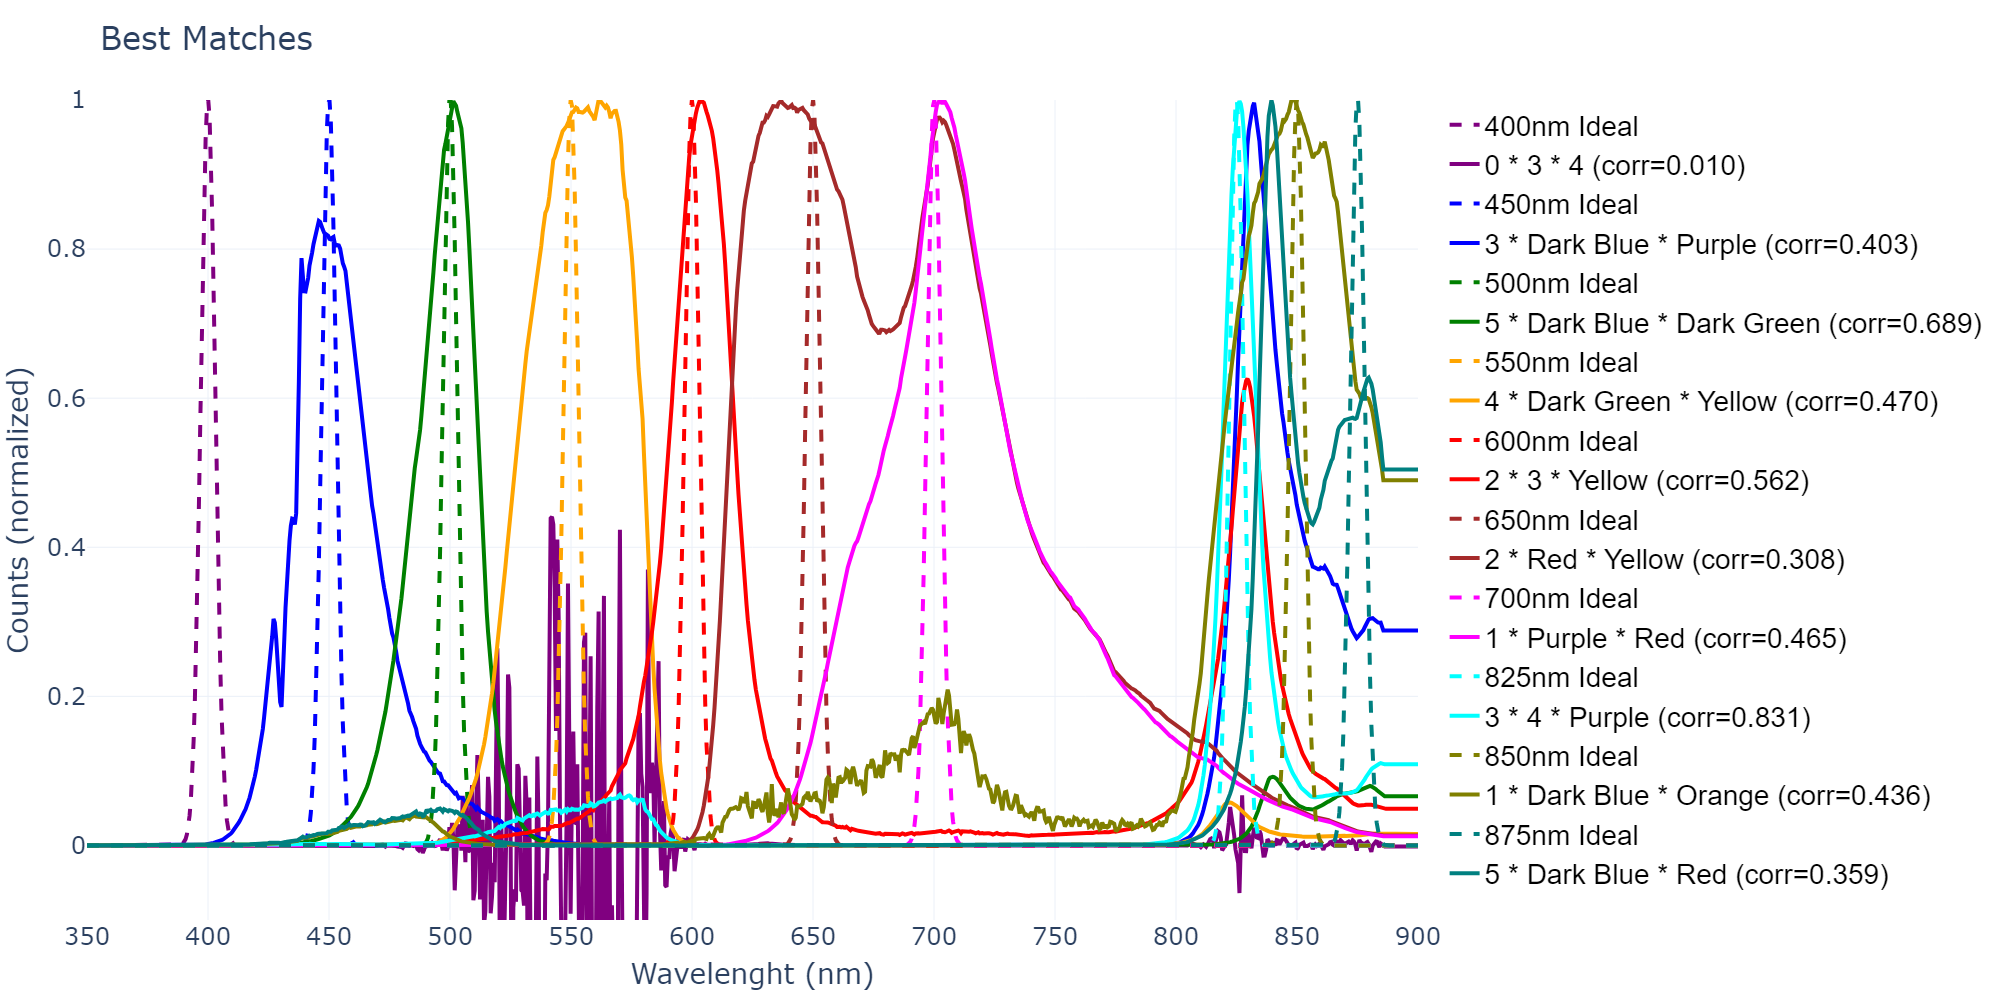
\includegraphics[trim=0mm 0mm 0mm 25mm, clip, width=1\textwidth]{Figures/C3/best_matches.png}
    \caption{Filter combinations (solid lines) with the highest correlation to their corresponding ideal curves (dashed lines). The shape and peak position of the selected combinations match the target profiles.}
    \label{fig:best_corr_combinations}
\end{figure}

\medskip

\noindent
Additionally, some combinations are selected experimentally, since the correlation-based method does not consider absolute transmittance. It is possible that the combination with the highest correlation \(r\) has very low transmittance, limiting its practical utility. Also, individual filters such as those centered at 532 and 633\,nm show good spectral performance. By combining the maximum correlation criterion with experimental validation, the final set of filters used for spectral characterization is selected.

\begin{figure}[htbp]
    \centering
    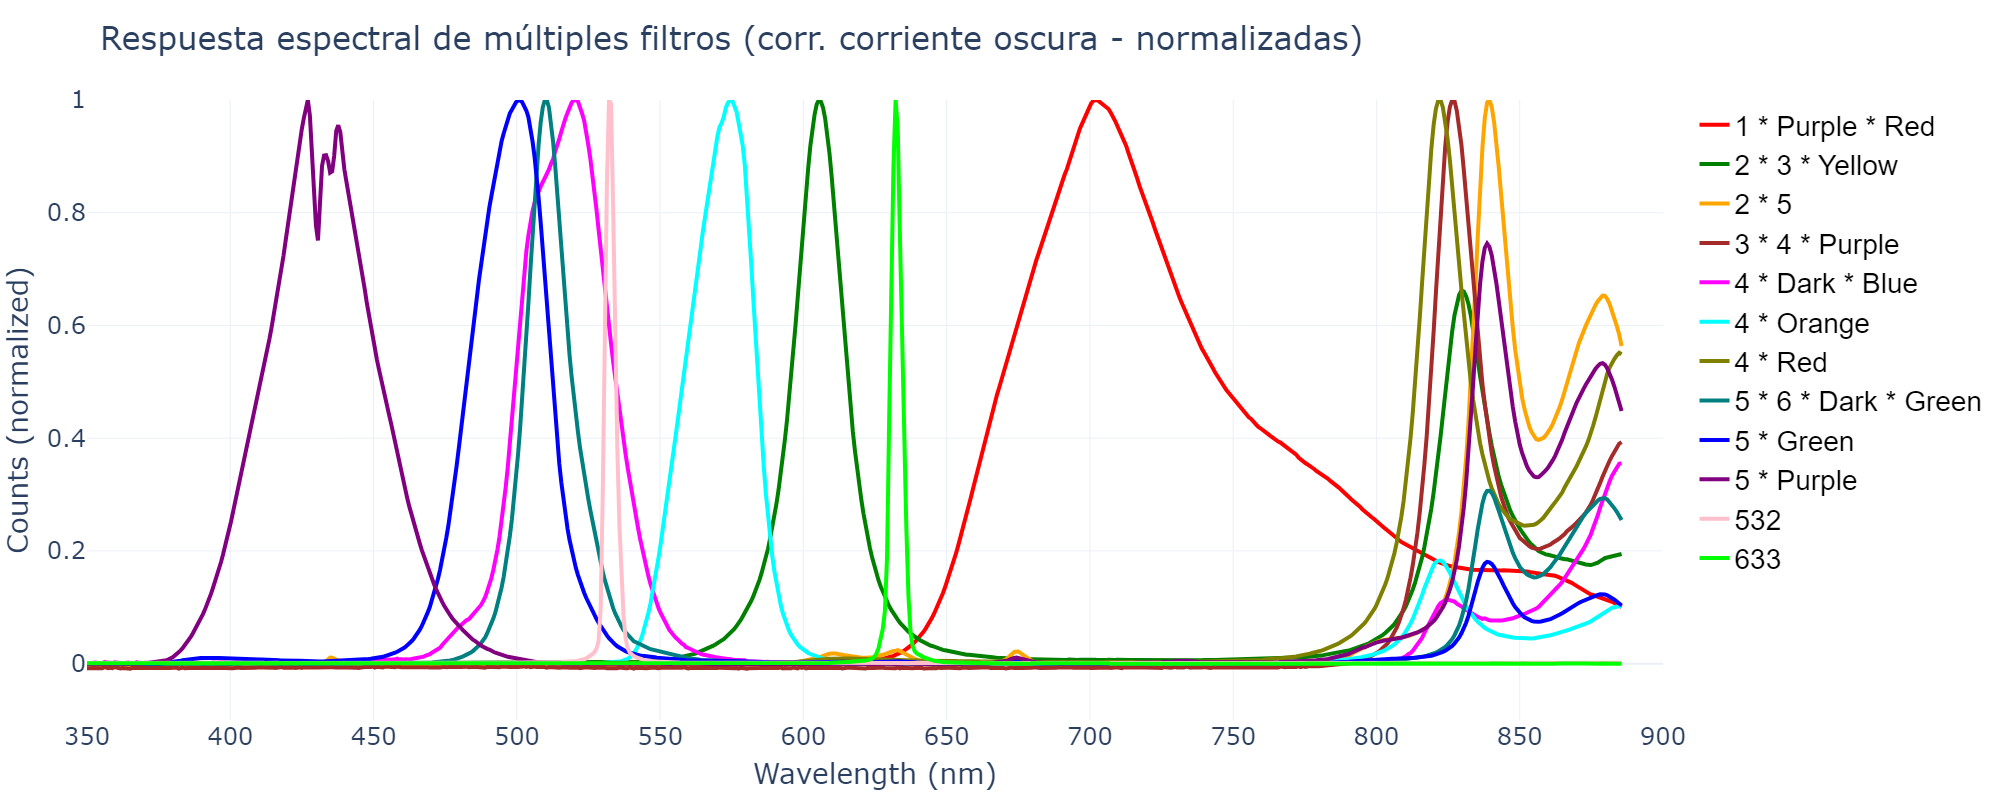
\includegraphics[width=1\textwidth]{Figures/C3/filt_select.png}
    \caption{Final filter selection used for spectral characterization of the optical systems. Includes both experimentally selected configurations and individual filters (532 and 633 nm) showing good correlation and transmittance.}
    \label{fig:selected_filters}
\end{figure}

\subsubsection{Determination of Central Wavelength, Bandwidth, and Optical Power of Selected Combinations}
\label{subsub:longitud_onda_central_potencia}

After defining the optimal combinations, the actual transmission spectra are measured using the minispectrometer to verify the effective central wavelength, resulting bandwidth, and transmitted optical power. This is essential to:

\begin{enumerate}
    \item Properly configure the optical power meter (which requires the central wavelength of the incoming radiation).
    \item Verify that the actual transmission curves are consistent with the numerically determined ones.
\end{enumerate}

The optical power transmitted by each selected combination is then measured using a power meter. To maintain consistency across measurements:

\begin{itemize}
    \item The tungsten lamp operates at its \textbf{maximum irradiance capacity}.
    \item For each combination, the power is measured at the previously determined central wavelength \(\lambda_0\).
\end{itemize}

The lowest power value among all combinations is used as the reference. This ensures that subsequent optical system measurements are performed under the same irradiance conditions, using neutral density filters to reduce irradiance in cases where power exceeds this reference.

\medskip

The bandwidth of the measured spectra for each selected filter is also calculated. Each spectrum is first normalized to have a maximum value of 1. The bandwidth is defined as the spectral interval where the signal reaches at least 50\% of its maximum value (i.e., the Full Width at Half Maximum, FWHM). For filters with multiple peaks, the main peak of interest is selected, usually corresponding to the expected region (e.g., NIR).

A Python script is developed that:

\begin{enumerate}
    \item Identifies the maximum peak of each normalized spectrum.
    \item Determines the wavelengths \(\lambda_{\text{left}}\) and \(\lambda_{\text{right}}\) where the spectral response falls to 50\% of the maximum.
    \item Calculates the bandwidth as:
    \[
    \text{FWHM} = \lambda_{\text{right}} - \lambda_{\text{left}}.
    \]
\end{enumerate}

Figure~\ref{fig:bandwidth_central} shows the central wavelength and FWHM of the selected filters, obtained through the described procedure. These parameters are key to assessing the system’s ability to discriminate spectral bands and for configuring the power meter accurately.

\begin{figure}[htbp]
    \centering
    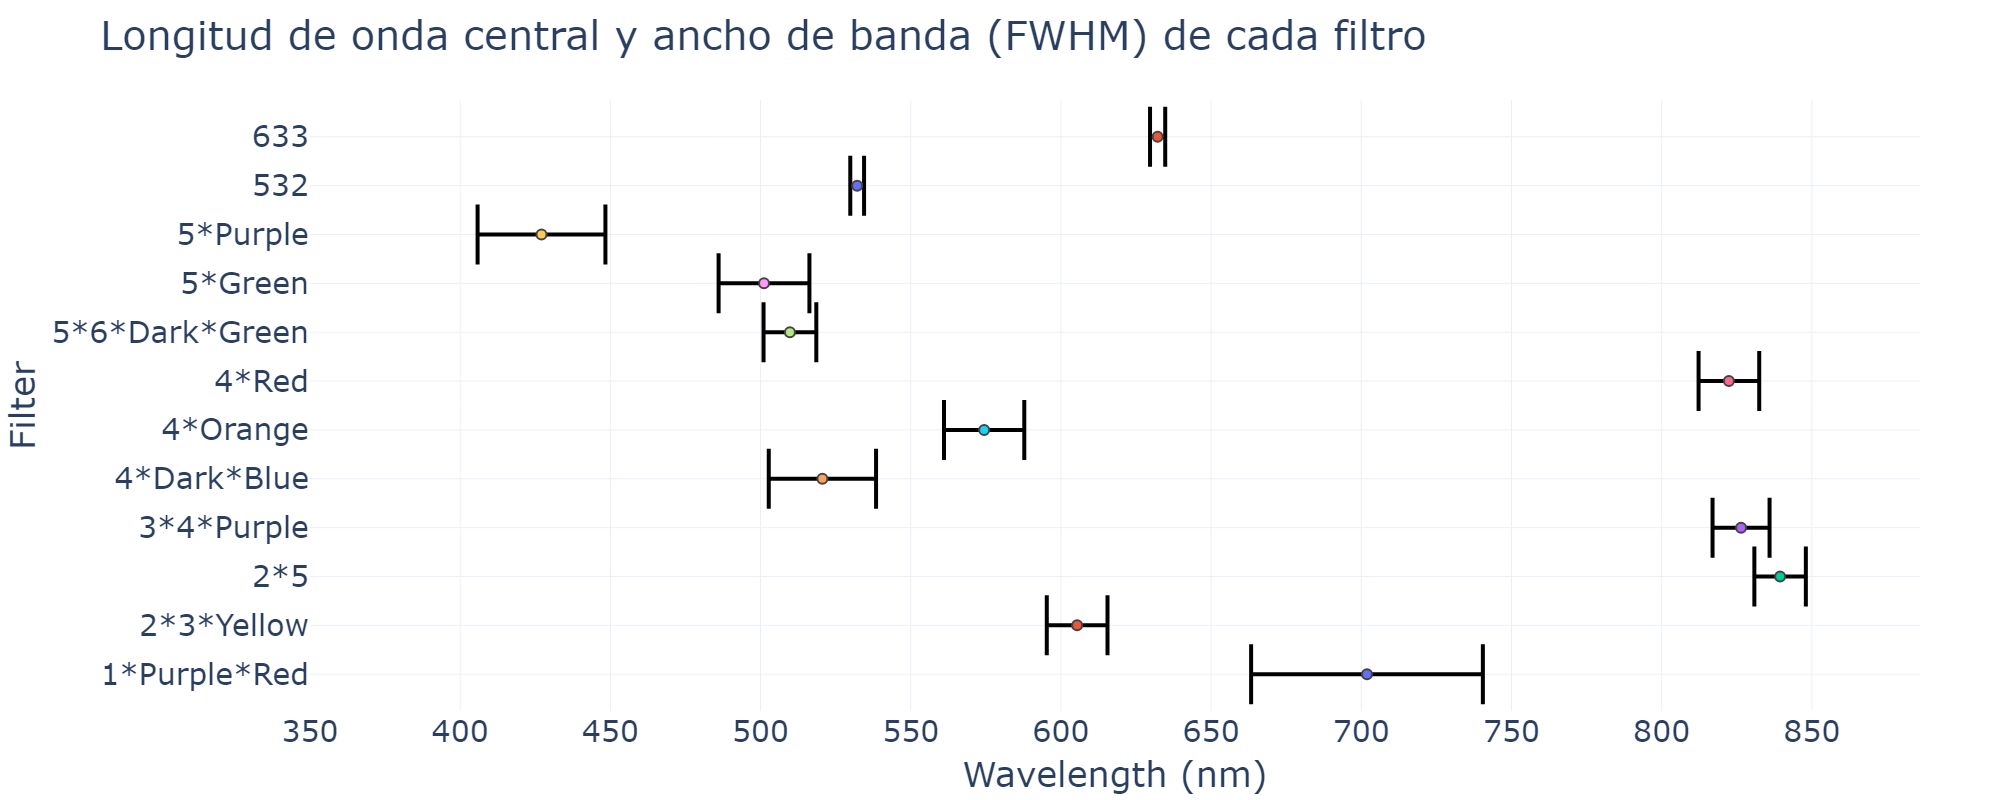
\includegraphics[trim=0mm 0mm 50mm 25mm, clip, width=1\textwidth]{Figures/C3/ancho de banda.png}
    \caption{Example of a normalized spectrum of a selected filter. The central wavelength and bandwidth (FWHM) are indicated, defined as the spectral range where the signal reaches 50\% of its maximum value.}
    \label{fig:bandwidth_central}
\end{figure}

\subsubsection{Image Capture with the Optical System Under Test}
\label{subsub:captura_sistemas_opticos}

Once the filter combinations are defined and the optical power is adjusted, the characterization of the target optical systems (e.g., an RGB system and/or a monochannel NIR system) is performed. The procedure is as follows:

\begin{enumerate}
    \item \textbf{Camera or sensor configuration:}
    \begin{itemize}
        \item \emph{Gain:} Set to $1$ for all measurements to avoid scaling differences between captures.
        \item \emph{Gamma:} Set to $1$ (linear) to suppress any internal nonlinearity curves.
        \item \emph{White balance:} In RGB cameras, the red and blue coefficients are set to $1$, and the green channel is also set to $1$ (if allowed by the firmware). This ensures that the camera does not apply color corrections.
    \end{itemize}
    
    \item \textbf{Use of neutral density filters (optional):} If the power exceeds the reference level, a neutral density filter is inserted into the lens tube after collimation. This ensures the same final power for all combinations.
    
    \item \textbf{Exposure time adjustment:} The exposure time is set to avoid image saturation. This value is recorded, since the system's response is \textbf{linearly proportional} to the integration time (see Equation~\ref{eq:modelo_lineal}).
    
    \item \textbf{Data capture:}
    \begin{itemize}
        \item For each selected filter combination, $50$ consecutive images of the optical system are acquired and saved in an uncompressed or minimally processed format. In this case, the format used is .npy.
        \item Additionally, $50$ dark current images are taken by completely covering the objective.
    \end{itemize}
    
    \item \textbf{Noise correction and averaging:}
    \begin{itemize}
        \item The average of the 50 dark current images is calculated, resulting in an image \(\mathbf{D}_{\text{prom}}\) that represents the system’s electronic offset.
        \item Each of the 50 illuminated captures is corrected by subtracting \(\mathbf{D}_{\text{prom}}\), thereby eliminating the dark current contribution.
        \item The 50 corrected images are then averaged, generating a single image \(\mathbf{I}_{\text{filt}}\) for each filter combination.
    \end{itemize}
    
    \item \textbf{Spectral response calculation:}
    \begin{itemize}
        \item For each averaged image (\(\mathbf{I}_{\text{filt}}\)), a \emph{response} metric is defined as the sum of all pixel values within the region of interest. In the case of an RGB camera, this sum can be calculated per channel (R, G, or B), or by converting the image to grayscale.
        \item In a monochromatic or NIR camera, the single available channel is used.
        \item The resulting value represents the system’s total response to the corresponding filter combination, associated with the calculated \(\lambda_0\).
    \end{itemize}
\end{enumerate}

\noindent
This process is repeated for each selected filter/sheet combination, generating a discrete spectral response map of the optical system, which relates the central wavelength to the response (as grayscale level sum or per channel).

